\documentclass[10pt,twocolumn,letterpaper]{article}

\usepackage[pagenumbers]{cvpr}

\usepackage{multirow}
\usepackage[table,xcdraw]{xcolor}
\usepackage{colortbl}
\usepackage{graphicx}
\usepackage{capt-of}
\usepackage{xspace}
\usepackage{times}
\usepackage{amsmath}
\usepackage{amssymb}
\usepackage{booktabs}
\usepackage{xpatch}
\usepackage{array}
\usepackage{multirow}
\usepackage{pifont}
\usepackage{enumitem}
\usepackage{bbm}
\usepackage{subcaption}
\usepackage{newtxtext}
\usepackage{amsthm}
\usepackage{algorithm}
\usepackage{algorithmicx}
\usepackage[noend]{algpseudocode}
\usepackage{placeins}

\usepackage{titletoc}

\theoremstyle{plain}
\newtheorem{theorem}{Theorem}[section]
\newtheorem{lemma}[theorem]{Lemma}
\newtheorem{proposition}[theorem]{Proposition}
\theoremstyle{remark}
\newtheorem*{remark}{Remark}

\renewcommand{\paragraph}[1]{\vspace{.5em}\noindent\textbf{#1.}}


\definecolor{Gray}{gray}{0.9}
\definecolor{cvprblue}{rgb}{0.21,0.49,0.74}
\usepackage[pagebackref,breaklinks,colorlinks,allcolors=cvprblue]{hyperref}

\title{Optimization-Guided Diffusion for Interactive Scene Generation}

\author{
Shihao Li$^{1,2,3}$ \quad
Naisheng Ye$^2$ \quad
Tianyu Li$^2$ \quad
Kashyap Chitta$^4$ \quad
Tuo An$^3$ \\
Peng Su$^5$ \quad
Boyang Wang$^1$ \quad
Haiou Liu$^1$ \quad
Chen Lv$^3$ \quad
Hongyang Li$^2$
\\[2mm]
$^1$ Beijing Institute of Technology \quad
$^2$ OpenDriveLab at The University of Hong Kong \quad  \\
$^3$ Nanyang Technological University \quad
$^4$ NVIDIA Research \quad
$^5$ Yinwang Intelligent Tech. Co. Ltd.
\\[1.5mm]
{
\hypersetup{urlcolor=Violet}
\href{https://opendrivelab.com/OMEGA}
{\texttt{{https://opendrivelab.com/OMEGA}}}
}
}



\begin{document}

\twocolumn[{
\maketitle
\vspace{-8pt}
\begin{center}
    \includegraphics[width=\linewidth]{sec/figs/Visualization_of_OMEGA.pdf}
    \vspace{-6pt}
    \captionof{figure}{\textbf{OMEGA \((\Omega)\).}
    Our plug-and-play, training-free guidance module can be dropped into existent diffusion-based driving scene generators to provide \textit{significantly more realistic, controllable, and interactive} traffic scenarios.
    \textbf{Top.} Our guidance produces diverse and realistic future scenarios from the same historical initialization, increasing the rate of physically and behaviorally valid scenes on both the nuPlan benchmark (used during the base model's training) and Waymo benchmark (zero-shot deployment) compared to unguided baselines.
    \textbf{Middle.} Controllability-conditioned generation synthesizes scenes where vehicles must reach predefined goal points (green flags) for one or multiple target agents, achieving precise behavioral control while maintaining natural interactions.
    \textbf{Bottom.} Finally, we enable adversarial scene generation, adaptively producing diverse attack scenarios without explicitly specifying attacker trajectories.
    Color transitions indicate the direction and speed of motion: \textbf{ego} (red gradient), \textbf{attacker} (yellow gradient), and \textbf{other vehicles} (blue gradient).
    }
    \label{fig:omega_visualization}
\end{center}
\vspace{4pt}
}]

{\let\thefootnote \relax
\footnote{
\hangindent=1.8em
Primary contact to Shihao Li \texttt{lishihao.shawn@gmail.com}
}}

\begin{abstract}
Realistic and diverse multi-agent driving scenes are crucial for evaluating autonomous vehicles, but safety-critical events which are essential for this task are rare and underrepresented in driving datasets. Data-driven scene generation offers a low-cost alternative by synthesizing complex traffic behaviors from existing driving logs. However, existing models often lack controllability or yield samples that violate physical or social constraints, limiting their usability. We present OMEGA, an optimization-guided, training-free framework that enforces structural consistency and interaction awareness during diffusion-based sampling from a scene generation model. OMEGA re-anchors each reverse diffusion step via constrained optimization, steering the generation towards physically plausible and behaviorally coherent trajectories. Building on this framework, we formulate ego–attacker interactions as a game-theoretic optimization in the distribution space, approximating Nash equilibria to generate realistic, safety-critical adversarial scenarios. Experiments on nuPlan and Waymo show that OMEGA improves generation realism, consistency, and controllability, increasing the ratio of physically and behaviorally valid scenes from 32.35\% to 72.27\% for free exploration capabilities, and from 11\% to 80\% for controllability-focused generation. Our approach can also generate $5\times$ more near-collision frames with a time-to-collision under three seconds while maintaining the overall scene realism.
\end{abstract}


\section{Introduction}
\label{sec:intro}

Generating realistic multi-agent driving scenes is essential for the development and evaluation of autonomous vehicles.
However, existing rule-based or physics-based simulators \cite{dosovitskiy2017carla, lopez2018microscopic} fall short: they can reproduce simple traffic patterns but often yield unrealistic or overly scripted interactions. Real-world datasets \cite{caesar2020nuscenes,caesar2021nuplan,dauner2024navsim,Cao2025CORL} also offer limited coverage, particularly for safety-critical long-tail events that are crucial for assessing robustness yet occur too infrequently to capture at scale \cite{liu2024curse}. 

These shortcomings highlight the need for a high-fidelity driving scene generator capable of producing realistic, diverse, and controllable multi-agent interactions, especially those involving rare behaviors, which has become an indispensable requirement for efficient and safe evaluation of autonomous driving systems \cite{lin2025model,ma2024unleashing,li2025mtgs,yang2025resim,tian2025simscale}.

To meet these requirements, researchers have turned to data-driven scene generation, which enables models to learn complex agent behaviors directly from large-scale driving datasets \cite{hu2024solving,seff2023motionlm,feng2022trafficgen}. Among these, diffusion models have shown remarkable potential in generating realistic multi-agent trajectories and coherent scene layouts, owing to their strong capacity to model high-dimensional, multi-modal distributions and produce samples consistent with empirical data \cite{jiang2024scenediffuser,huang2024versatile}. Despite this success, existing diffusion-based generators face two key limitations.

First, while the learned denoising network implicitly encodes physical and social constraints from data during training, such structure often degrades during inference. As noise is progressively removed, small inconsistencies can accumulate across steps, leading to trajectories that violate kinematic feasibility, social compliance, or interaction logic. These physically or behaviorally inconsistent samples reduce the credibility of generated scenes and limit their utility for downstream safe evaluation.

Second, long-tail and adversarial interactions lie in low-density regions of naturalistic datasets and are therefore underrepresented during training. Consequently, learned models gravitate toward dominant motion patterns and struggle to directly sample rare but safety-critical interactions. Prior diffusion methods introduce guidance via reinforcement-learned classifiers \cite{xie2024advdiffuser}, manually designed behavior-shaping objectives \cite{xu2025diffscene, zhong2022guided}, or pre-specified goal conditions \cite{zhou2025decoupled, jiang2023motiondiffuser}. These strategies either require retraining auxiliary networks or rely on case-by-case guidance functions that demand domain expertise, which limits scalability and generalization across scenarios.

To address these limitations, we introduce OMEGA, a training-free framework that incorporates structural constraints and strategic intent into diffusion-based driving scene generation. OMEGA formulates each reverse diffusion step as a conditional sampling process anchored on the estimated clean sample and performs numerical optimization within a KL-bounded trust region to re-anchor the mean of the reverse transition distribution. This optimization-guided formulation progressively steers the reverse Markov chain toward physically consistent and behaviorally coherent trajectories, improving structural fidelity without retraining or altering the backbone diffusion model.

To improve interaction realism, we introduce a two-phase noise scheduling scheme. Coarse denoising over full trajectories establishes the macro-level layout, while fine-grained, time-indexed denoising enhances reactivity and enforces physically feasible multi-agent interactions.

Building on this foundation, we further introduce OMEGA$_\mathrm{Adv}$, a sensitivity-enhanced  adversarial generator inspired by \cite{fiacco1983introduction,spica2020real}. It models attacker--ego interactions as a distributional optimization game. The ego agent seeks to maintain natural, feasible behavior, while the attacker, using a sensitivity term that predicts how the ego will react to impending collision-avoidance constraints, seeks to maximally perturb the ego within the learned data distribution. This formulation enables the adaptive generation of realistic yet challenging driving scenarios without retraining any components or manually prescribing attacker trajectories or target points. Our contributions include:

\begin{itemize}
    \item Optimization-guided diffusion sampling. A plug-and-play, training-free method that re-anchors each reverse step via constrained optimization, enforcing structural consistency and stable diffusion guidance.
    \item Two-phase noise scheduling for interaction fidelity, ensuring macro-level plausibility with fine-grained reactivity, enabling context-aware and dynamically coordinated multi-agent scene evolution.
    \item Sensitivity-enhanced adversarial generation. A game-thoretic formulation for ego--attacker interactions yielding realistic yet challenging scenarios.
    \item Comprehensive empirical results. OMEGA reduces collisions and off-road rates while improving kinematic feasibility over baselines. It raises scene validity on nuPlan by about 40 points and on Waymo (zero-shot) by about 20 points, and delivers a further 69-point gain in controllability under user-specified intents. It is also capable of generating $5\times$ more near-collision frames under the adversarial scene generation setting.
\end{itemize}

\section{Related Work}
\label{sec:related}

\paragraph{Diffusion models for conditioned generation}
A spectrum of generative architectures has been explored to address driving scenario generation, encompassing autoregressive approaches~\cite{seff2023motionlm,hu2024solving} and diffusion-based frameworks~\cite{jiang2024scenediffuser,tan2025scenediffuser++,zhou2025decoupled,chitta2024sledge}. The latter offers greater flexibility for joint distribution modeling and controllable conditional synthesis. However, existing guidance mechanisms used in trajectory- and scene-level diffusion models remain inherently fragile. DPS-style Jacobian guidance~\cite{zheng2025diffusion, chung2022diffusion} relies on a first-order linearization of the highly nonlinear noise–state mapping, often yielding oscillatory or high-variance gradients. CTG~\cite{zhong2022guided} approximates conditional scores using predicted reverse-step means, but trajectory-level objectives defined in the clean space become unreliable when extrapolated to high-noise samples, yielding low-SNR gradients that distort the descent direction. Geometry-constrained methods such as GHC~\cite{jiang2024scenediffuser} enforce hard clipping or projection during denoising, introducing discontinuities that disrupt the smoothness and distributional coherence of the generative process. Overall, these guidance strategies introduce external biases beyond the original reverse diffusion chain. Since the model is iteratively applied to its own outputs, unstable or overly strong guidance can cause accumulated deviations, leading to distribution shifts or even mode collapse.


\paragraph{Safety-critical scenario generation}
Generating high-fidelity, safety-critical driving scenarios is paramount for the robust training and evaluation of autonomous driving systems~\cite{Hu2023CVPR,Chen2024PAMI,liu2025reinforced}. Certain approaches employ adversarial learning \cite{zhang2023cat,feng2023dense}, which trains surrounding agents to adversarially interact with the ego vehicle. Gradient-based perturbation methods, including KING~\cite{hanselmann2022king} and AdvSim~\cite{wang2021advsim}, modify background trajectories, or re-simulate sensor data, to induce critical states while preserving physical plausibility. AdvDiffuser \cite{xie2024advdiffuser} injects gradients into the denoising process from an auxiliary collision reward model, steering the diffusion updates toward adversarial trajectories. Nexus~\cite{zhou2025decoupled} leverages manually specified goal-condition inpainting to guide selected agents toward pre-defined outcomes, enabling targeted critical events under explicitly defined goal configurations. In contrast to these approaches, our method, OMEGA$_\mathrm{Adv}$, generates adversarial scenarios through formulating a distributional game in the optimization guided denoising process, enabling realistic yet safety-critic scenario generation.

\begin{figure*}[t]
    \centering
    \includegraphics[width=\linewidth]{sec/figs/OMEGA.pdf}
    \vspace{-10pt}
    \caption{\textbf{Standard diffusion sampling (top) vs. our optimization-guided OMEGA (bottom).}  
    We re-anchor each reverse diffusion step via constrained optimization within a KL-bounded trust region, steering the Markov chain towards behaviorally coherent samples.}
    \label{fig:omega}
\end{figure*}



\section{Method}
\label{sec:method}

\subsection{Preliminary}

\paragraph{Diffusion models}
Diffusion models~\cite{sohl2015deep, ho2020denoising, dhariwal2021diffusion, song2021denoising} are likelihood-based generative models that map a simple Gaussian prior to complex data distributions through sequential denoising. Given $x_0 \!\sim\! q(x_0)$, the \textit{forward diffusion} adds Gaussian noise with variance $\beta_t \in (0, 1)$ at each step to obtain a sequence of intermediate states $x_1, \ldots, x_T$. The analytic marginal distribution of conditioned on $x_0$ is:
\begin{equation}
\begin{aligned}
q(x_t \mid x_0)
&= \mathcal{N}\!\big(\sqrt{\bar{\alpha}_t}\,x_0,\; (1-\bar{\alpha}_t)I\big), \\
x_t
&= \sqrt{\bar{\alpha}_t}\,x_0 + \sqrt{1-\bar{\alpha}_t}\,\epsilon,
\end{aligned}
\label{eq:xt_x0}
\end{equation}
where \(\alpha_t = 1 - \beta_t\), \(\bar{\alpha}_t = \prod_{s=1}^t \alpha_s\), and \(\epsilon \sim \mathcal{N}(0, I)\).


Starting from pure noise $x_T \!\sim\! \mathcal{N}(0,I)$, the \textit{reverse process} reconstructs data from noise and is modeled as a Gaussian transition:
\begin{equation}
p_\theta(x_{t-1}\mid x_t)
= \mathcal{N}\!\big(\mu_\theta(x_t, t),\, \Sigma_\theta(x_t, t)\big),
\end{equation}
where in DDPMs~\cite{ho2020denoising} the variance $\Sigma_\theta$ is fixed as $\sigma_t^2 I$, 
and the network learns to predict the noise term $\epsilon_\theta(x_t, t)$ that perturbed $x_0$ to obtain $x_t$.
After training, samples are generated by iteratively applying this reverse transition:
\begin{equation}
x_{t-1}
= \frac{1}{\sqrt{\alpha_t}}
\!\left(x_t - \frac{1 - \alpha_t}{\sqrt{1 - \bar{\alpha}_t}}\,
\epsilon_\theta(x_t, t)\!\right)
+ \sigma_t z,
\label{eq:ddpm_sample}
\end{equation}
where $z \sim \mathcal{N}(0, I)$ and $t = T, \ldots, 1$. Here, $\beta_t$ denotes the noise schedule, $\alpha_t = 1 - \beta_t$ is the retained signal coefficient, and $\bar{\alpha}_t$ is its cumulative product controlling the noise level.

\paragraph{Problem formulation}
We represent a traffic scene as a spatiotemporal tensor \( x \in \mathbb{R}^{A \times \mathcal{T} \times D} \)
where \( A \) denotes the number of interacting agents, \( \mathcal{T} \) the total number of physical timesteps, and \( D \) the state dimension including position, heading, velocity, and physical size. 
A binary validity mask \( m \in \mathbb{B}^{A \times \mathcal{T}} \) indicates each agent’s existence over time, accounting for dynamic entries and exits.
Following prior works \cite{jiang2024scenediffuser, zhou2025decoupled}, we formulate driving scene generation as a multi-agent inpainting problem over $x$.
Given an inpainting mask \( \tilde{m} \in \mathbb{B}^{A \times \mathcal{T} \times D} \) and its corresponding context values \( \bar{x} = \tilde{m} \odot x \), the diffusion model learns to reconstruct the unobserved elements of \( x \) conditioned on both local spatiotemporal and global scene information.
The given context may include arbitrary known elements of $x$, such as all agents’ past trajectories or designated future goals for specific agents. 
The effective target region for generation corresponds to valid but unobserved elements \( m \odot (1-\tilde{m}) \), representing future state of existing agents or newly introduced ones. Within this formulation, the diffusion model iteratively refines the scene tensor through denoising, progressively completing the partially observed scene toward a coherent multi-agent configuration. 


\subsection{Optimization-Guided Constrained Diffusion}
\label{sec:omega}

\vspace{2pt}
\paragraph{Anchored reverse transition}
In the standard diffusion sampling process, the model predicts the injected noise $\epsilon_\theta(x_t, t)$ at each step, from which an approximate clean estimate corresponding to the noisy state \(x_t\) can be obtained via \cref{eq:xt_x0}:
% \kc{incorrect equation number?}:
\begin{equation}
\tilde{x}_0 = \frac{x_t - \sqrt{1-\bar{\alpha}_t}\,\epsilon_\theta(x_t, t)}{\sqrt{\bar{\alpha}_t}}.
\label{eq:x0_estimate}
\end{equation}
Substituting $\tilde{x}_0$ into the reverse kernel, the posterior distribution of $x_{t-1}$ given $x_t$ can be expressed as:
\begin{equation}
p_\theta(x_{t-1} \mid x_t)
= \mathcal{N}\!\big(x_{t-1};\, A_t \tilde{x}_0 + C_t x_t,\, \sigma_t^2 I\big),
\label{eq:reverse_kernel}
\end{equation}
where $A_t = \frac{(1 - \alpha_t)\sqrt{\bar{\alpha}_{t-1}}}{1 - \bar{\alpha}_t}$ and 
$C_t = \frac{\sqrt{\alpha_t}(1 - \bar{\alpha}_{t-1})}{1 - \bar{\alpha}_t}$ 
are deterministic coefficients determined by the variance schedule.  
Since $x_t$, $A_t$, and $C_t$ are fixed at each step, the conditional distribution of $x_{t-1}$ is fully characterized by the model-estimated clean sample $\tilde{x}_0$.  
For convenience, we denote this Gaussian transition as \( Q_t(\tilde{x}_0) \),  
indicating that the reverse kernel is anchored on $\tilde{x}_0$ while its variance and linear coefficients are fixed by $(x_t, t)$.

Accordingly, \cref{eq:ddpm_sample} can be rewritten as:
\begin{equation}
x_{t-1}
= \underbrace{A_t \tilde{x}_0}_{\text{regression term}}
+ \underbrace{C_t x_t}_{\text{inertia term}}
+ \underbrace{\sigma_t z}_{\text{noise term}}.
\end{equation}
This update can be decomposed into three interpretable components:
(i) a \textbf{regression term} ($A_t \tilde{x}_0$) that pulls the sample toward the model-predicted clean state,
(ii) an \textbf{inertia term} ($C_t x_t$) that preserves continuity with the current noisy state and stabilizes transitions across steps,
and (iii) a \textbf{noise term} ($\sigma_t z$) that maintains sample diversity through controlled stochasticity.
Together, these components describe a reverse process that iteratively moves $x_t$ toward $\tilde{x}_0$, progressively refining the sample trajectory until convergence to the data manifold.
This perspective highlights that each reverse diffusion step constitutes a \textit{conditional sampling process anchored on the predicted clean sample}, where $\tilde{x}_0$ defines the denoising target guiding the evolution of the Markov chain.

\vspace{3pt}
\paragraph{Optimization-guided re-anchoring}
While the predicted clean sample $\tilde{x}_0$ defines the local denoising direction inferred from the learned dynamics, it is derived purely through data-driven regression and thus may deviate from regions consistent with structural or behavioral priors, gradually drifting away from the manifold of physically and behaviorally coherent samples.

\begin{figure*}[!t]
    \centering
    \includegraphics[width=\linewidth]{sec/figs/Toy_Example.pdf}
    \vspace{-15pt}
    \caption{\textbf{Toy example illustrating the effect of OMEGA on the generative manifold.}  
    We design a simple two-dimensional generation task to visualize how our method influences the learned data manifold.
    (a) Without any guidance, the diffusion model approximates the target data distribution and generates samples along its intrinsic manifold.
    (b) Using only the guidance objective $R(x)$ pulls samples excessively toward the guidance point, thereby distorting local geometry.
    (c) Combining with a KL constraint yields controlled adaptation toward the guidance point while preserving learned manifold fidelity.
    Details are provided in Appendix~\ref{sec:toy}.
}
    \label{fig:toy_exm}
\end{figure*}


To explicitly regularize this evolution, OMEGA introduces an optimization-guided refinement of the anchor (Fig.~\ref{fig:omega}), redefining each reverse transition as a new distribution $P_t(\hat{x}_0)$ whose mean is adaptively adjusted within a bounded divergence from the original kernel:
\begin{equation}
\begin{aligned}
P_t(\hat{x}_0) &= \mathcal{N}(A_t \hat{x}_0 + C_t x_t,\, \sigma_t^2 I), \\
\text{s.t.} \quad 
&\mathrm{KL}\!\big(P_t(\hat{x}_0) \,\Vert\, Q_t(\tilde{x}_0)\big) \le \kappa_t.
\end{aligned}
\end{equation}
The optimized anchor $\hat{x}_0$ is obtained by solving a constrained maximization problem:
\begin{equation}
\begin{aligned}
\hat{x}_0
= \arg\max_{x}\;
&\Big[
\lambda_t R(x)
- \, \mathrm{KL}\!\big(P_t(x) \,\Vert\, Q_t(\tilde{x}_0)\big)
\Big], \\
\text{s.t.}\quad
&\mathrm{KL}\!\big(P_t(x) \,\Vert\, Q_t(\tilde{x}_0)\big)
\le \kappa_t.
\end{aligned}
\label{eq:omega_opt}
\end{equation}
Here, \(R(x)\) serves as a differentiable objective that encodes structural and behavioral preferences guiding the generation process, while the KL term defines a trust region that regularizes deviation from the model’s learned manifold.
As illustrated by the toy example in Fig.~\ref{fig:toy_exm}, this constraint prevents excessive drift or mode collapse, stabilizing the denoising dynamics and preserving fidelity to the generative manifold encoded by the pretrained diffusion model.
Through this balance, the sampler implicitly shifts the mean of the reverse transition toward constraint-consistent regions, adapting its trajectory while maintaining distributional coherence within the generative space.

OMEGA guides the denoising process through distributional re-anchoring, softly steering each reverse step toward constraint-consistent regions while preserving the learned generative manifold. By iteratively optimizing the anchor $\hat{x_0}$ and resampling from $P\left(\hat{x}_0\right)$, the process progressively re-aligns the reverse Markov chain with both the model’s learned data distribution and the imposed structural priors, enabling structural yet distributionally coherent generation.


\paragraph{Equivalent euclidean formulation}
Since the anchor $\hat{x}_0$ directly corresponds to the joint future trajectories of all agents in the scene, it admits a physically meaningful interpretation in the optimization space. We represent \(R(x)\) as a structured objective \(r(x)\) equipped with equality and inequality constraints \(h(x)=0\) and \(g(x)\le0\), encoding different levels of structural and behavioral priors. 
Here, \(r(x)\) captures trajectory-level preferences such as smoothness, 
\(h(x)=0\) enforces equality relations such as kinematic feasibility,  
and \(g(x)\le0\) defines inequality conditions such as collision avoidance or boundary adherence.

By substituting the Gaussian forms of \(P_t(x)\) and \(Q_t(\tilde{x}_0)\) into \cref{eq:omega_opt},  
the optimization can be explicitly written in the Euclidean domain as:
\begin{equation}
\begin{aligned}
\hat{x}_0
&=\arg\max_x\;
\lambda_t\, r(x)
-\frac{A_t}{2\sigma_t^2}\,\|x-\tilde{x}_0\|_2^2, \\
&\text{s.t.}\;\;
\|x-\tilde{x}_0\|_2
\le
\sqrt{2\kappa_t}\,\frac{\sigma_t}{|A_t|}, \\
&\qquad h(x)=0,\quad g(x)\le0.
\end{aligned}
\label{eq:euclid-form}
\end{equation}


This equivalent formulation shows that the KL-divergence constraint in \cref{eq:omega_opt} translates into an adaptive Euclidean trust region,  
whose radius scales proportionally with the diffusion variance \(\sigma_t\).  
Conceptually, the effective trust region scales with the diffusion variance.
Early reverse steps, dominated by stochastic uncertainty, allow the optimization to explore a wider subset of feasible configurations, while subsequent steps, operating under lower variance, restrict updates to a local vicinity of the data manifold,
thereby promoting convergence stability and preserving consistency with the learned generative dynamics.


\subsection{Two-phase Noise Scheduling}
\label{sec:noise_schedule}

To balance global coherence and local responsiveness in multi-agent scene generation,  
we introduce a two-phase noise scheduling scheme, termed \textit{Warmup} and \textit{Rolling-Zero}, which jointly enhance interaction fidelity and temporal stability, as shown in \cref{fig:noise_schedule}.

\paragraph{Warmup phase}
The Warmup phase performs full-sequence denoising over each agent’s trajectory under a gradually decreasing noise schedule.  
This global optimization establishes macro-level spatial organization and dynamic plausibility, ensuring smooth and kinematically coherent motion over the entire horizon. 
By treating the temporal sequence as a unified objective, Warmup suppresses autoregressive drift and stabilizes long-horizon trends, then halts at a low-noise regime to provide a well-posed initialization for subsequent refinement.

\paragraph{Rolling-Zero phase}
Operating in the low-noise regime produced by Warmup, the Rolling-Zero phase advances a time-indexed denoising window, progressively removing the residual noise that Warmup intentionally leaves unremoved. At each step, one frame is refined conditioned on previously cleaned states, enabling frame-level adaptation to evolving inter-agent interactions and environmental cues. 

\paragraph{Phase coupling for interaction fidelity}
The two phases are hierarchical and complementary: Warmup provides a globally stable foundation for layout and motion smoothness, whereas Rolling-Zero restores fine-grained reactivity by refining the remaining uncertainty at the frame level. 
In practice, objectives are scheduled accordingly: during Warmup, agents are guided independently under kinematic and smoothness priors; during Rolling-Zero, inter-agent guidance terms are introduced and evaluated against the clean states from the previous step. This progressive coupling reduces the complexity of joint multi-agent optimization while enhances responsiveness, and naturally supports parallel computation. 



\begin{figure}[t]
    \centering
    \includegraphics[width=\columnwidth]{sec/figs/Two-phase_noise_scheduling.pdf}
    \vspace{-12pt}
    \caption{\textbf{Illustration of two-phase noise scheduling.} Darker blue means higher noise, lighter blue means lower noise.}
    \vspace{-12pt}
    \label{fig:noise_schedule}
\end{figure}

\subsection{Sensitivity-Enhanced Adversarial Generation}
\label{sec:omega_se}

Building upon the OMEGA formulation, OMEGA$_\mathrm{Adv}$ extends it to adversarial scene generation by formulating a sensitivity-enhanced distributional game between the ego vehicle \(e\) and an attacker \(a\). While the ego aims to preserve feasibility and realism within the learned generative manifold, the attacker seeks to induce maximal perturbations that remain distributionally consistent, thereby exposing safety-critical yet physically plausible interactions. This formulation enables adversarial scenario synthesis directly within the learned generative manifold, without retraining or external trajectory scripting.

Following this distributional game setup, both participants perform constrained optimization: the ego strives to maintain realistic feasibility:
\begin{equation}
\begin{aligned}
\hat{x}_0^e = 
&\arg\max_{x^e} \; J^e(x^e) \\
\text{s.t.}\quad
&\|x^e - \tilde{x}_0^e\|_2 \le \rho_t, \;
h(x^e)=0,\; g(x^e)\le0, \\
&\gamma_e(x^e,x^a)\le 0,
\end{aligned}
\label{eq:ego_opt}
\end{equation}
while the attacker perturbs ego behavior by solving:
\begin{equation}
\begin{aligned}
\hat{x}_0^a =
&\arg\max_{x^a} \; J^a(x^a) - \alpha J^e(x^e) \\
\text{s.t.}\quad
&\|x^a - \tilde{x}_0^a\|_2 \le \rho_t, \;
h(x^a)=0,\; g(x^a)\le0, \\
&\gamma_a(x^a,x^e)\le 0.
\end{aligned}
\label{eq:attacker_opt}
\end{equation}
Here, \(J^e\) and \(J^a\) share the same structural form as \cref{eq:euclid-form}, 
ensuring consistency with the learned generative manifold, 
while \(\alpha>0\) balances the attacker’s aggressiveness against realism. 
The pairwise safety constraint \(\gamma(x^e,x^a)\) couples the two subproblems, 
inducing a noncooperative differential game where each player’s feasible set depends on the other’s strategy and is activated only within their respective responsibility regions.


\begin{table*}[!t]
\centering
\caption{%
    \textbf{Free-exploration scene generation results on nuPlan and zero-shot evaluation on Waymo.} 
    Oracle refers to original logs in the dataset.
    N-Dist. (nearest-agent distance distribution JSD, $10^{-3}$), 
    L-Dev. (lateral deviation distribution JSD, $10^{-3}$), 
    A-Dev. (angular deviation distribution JSD, $10^{-3}$), 
    Spd. (speed distribution JSD, $10^{-3}$), 
    P-Ag./P-Sc. (per-agent/per-scene rate), 
    and overall Scene Valid Rate (no collision/off-road/kinematic violation). 
    $\downarrow$ indicates lower is better; $\uparrow$ indicates higher is better.
}
\vspace{-9pt}
\label{tab:comparison}
\resizebox{\textwidth}{!}{
\begin{tabular}{c|l|cccc|cc|cc|cc|>{\columncolor{Gray}}c}
\toprule
& & \multicolumn{4}{c|}{\textbf{Distributional JSD}} & \multicolumn{2}{c|}{\textbf{Collision Rate}} & \multicolumn{2}{c|}{\textbf{Off-road Rate}} & \multicolumn{2}{c|}{\textbf{Kinematic Feasibility}} & \textbf{Valid Rate} \\
\multirow{-2}{*}{\textbf{Dataset}} & \multirow{-2}{*}{\textbf{Method}} & N-Dist. $\downarrow$ & L-Dev. $\downarrow$ & A-Dev. $\downarrow$ & Spd. $\downarrow$ & P-Ag. $\downarrow$ & P-Sc. $\downarrow$ & P-Ag. $\downarrow$ & P-Sc. $\downarrow$ & P-Ag. $\uparrow$ & P-Sc. $\uparrow$ & P-Sc. $\uparrow$ \\
\midrule
\multicolumn{1}{l|}{} & Oracle & 0.000 & 0.000 & 0.000 & 0.000 & 0.38& 13.62& 0.00 & 0.00 & 97.40 & 81.22 & 71.67 \\
\multicolumn{1}{l|}{} & D. Policy~\cite{chi2025diffusion} & 0.701 & 0.056 & 0.423 & 0.369 & 1.19& 36.58& 4.37 & 39.47 & 98.46 & 87.18 & 34.49 \\
\multicolumn{1}{l|}{} & SceneD.~\cite{jiang2024scenediffuser} & 0.933 & 0.046 & 0.395 & \textbf{0.234} & 1.19& 37.80& 4.84 & 41.68 & 98.48 & 86.96 & 33.27 \\
\multicolumn{1}{l|}{} & Nexus~\cite{zhou2025decoupled} & 1.162 & 0.041 & 0.461 & 1.018 & 1.41& 43.12& 4.70 & 40.13 & 98.72 & 88.63 & 32.35 \\
\multicolumn{1}{l|}{\multirow{-5}{*}{nuPlan}} & Nexus-$\Omega$ & \textbf{0.203} & \textbf{0.025} & \textbf{0.081} & 0.333 & \textbf{0.19}& \textbf{17.36} & \textbf{0.91} & \textbf{10.39} & \textbf{99.19} & \textbf{91.91} & \textbf{72.27} \\
\midrule
& Oracle & 0.000 & 0.000 & 0.000 & 0.000 & 0.22 & 7.47 & 0.00 & 0.00 & 99.77 & 96.33 & 89.33 \\
& D. Policy~\cite{chi2025diffusion} & 0.034 & 0.026 & 0.081 & 0.229 & 0.35& 19.23& 1.04 & 11.35 & 98.86 & 86.74 & 64.55 \\
& SceneD.~\cite{jiang2024scenediffuser} & 0.077 & 0.022 & 0.148 & 0.249 & 0.39& 22.94 & 1.22 & 12.18 & 98.81 & 86.57 & 61.01 \\
& Nexus~\cite{zhou2025decoupled} & 0.081 & 0.022 & 0.154 & 0.251 & 0.38 & 22.65 & 1.23 & 12.30 & 98.76 & 86.08 & 61.71 \\
\multirow{-5}{*}{Waymo} & Nexus-$\Omega$ & \textbf{0.019} & \textbf{0.015} & \textbf{0.050} & \textbf{0.198} & \textbf{0.18} & \textbf{11.43} & \textbf{0.37} & \textbf{4.32} & \textbf{99.40} & \textbf{92.65} & \textbf{81.95} \\
\bottomrule
\end{tabular}
}
\vspace{-6pt}
\end{table*}

\paragraph{Sensitivity-enhanced iterative best response}
Directly solving the joint optimization in Eqs. (\ref{eq:ego_opt})-(\ref{eq:attacker_opt}), which constitutes a noncooperative differential game, is computationally prohibitive. To approximate its Nash equilibrium efficiently, we adopt a sensitivity-enhanced iterative best response (SE-IBR) scheme \cite{spica2020real}. Starting from the model-predicted anchors \(\tilde{x}_0^e\) and \(\tilde{x}_0^a\) as initial strategies, the ego and attacker alternately update their clean anchors as best responses to each other, iterating until convergence.  

Let \(x^{a(l-1)}\) denote the attacker’s previous anchor and \(x^{e(l)}\) the ego’s current optimized response. 
Since the ego’s optimal value \(J^{e*}(x^a)\) implicitly depends on the attacker’s decision \(x^a\),  SE-IBR characterizes its local sensitivity around \(x^{a(l-1)}\) via a first-order Taylor approximation:
\begin{equation}
J^{e*}(x^a) \approx J^{e*}\!\big(x^{a(l-1)}\big)
+ \left.\frac{\mathrm{d} J^{e*}}{\mathrm{d} x^a}\right|_{x^{a(l-1)}}\!(x^a - x^{a(l-1)}).
\label{eq:linearize}
\end{equation}
Using the Karush-Kuhn-Tucker (KKT) optimality conditions of the ego’s constrained problem (\ref{eq:ego_opt}),  the sensitivity of \(J^{e*}\) with respect to the attacker’s decision can be expressed as:
\begin{equation}
\left.\frac{\mathrm{d} J^{e*}}{\mathrm{d} x^a}\right|_{x^{a(l-1)}} 
\approx -\mu^{e(l)} 
\left.\frac{\partial \gamma_e}{\partial x^a}\right|_{(x^{a(l-1)},x^{e(l)})},
\label{eq:sensitivity}
\end{equation}
where \(\mu^{e(l)}\!\ge\!0\) is the KKT multiplier associated with ego’s active collision constraint \(\gamma_e(x^a,x^e)\le0\).  
Substituting Eqs.~(\ref{eq:linearize})-(\ref{eq:sensitivity}) yields the attacker’s sensitivity-enhanced update:
\begin{equation}
\begin{aligned}
\hat{x}_0^a \approx\; &\arg\max_{x^a}\; 
J^a(x^a) 
+ \alpha \mu^{e(l)} 
\left.\frac{\partial \gamma_e}{\partial x^a}\right|_{(x^{a(l-1)},x^{e(l)})}
x^a
 \\
\text{s.t.}\quad 
&\text{(same constraints as (\ref{eq:attacker_opt})).}
\end{aligned}
\label{eq:attacker_seibr}
\end{equation}


When the ego’s avoidance constraint becomes active (i.e. \(\mu^{e(l)}>0\)), the attacker acquires a directional incentive proportional to $\partial \gamma_e/{\partial x^a}$, which encourages attacker motions that decrease the signed-distance in the ego--attacker interaction space. 
Intuitively, this steers the attacker toward maneuvers that effectively reduce the ego’s feasible maneuvering set and thus elicit a reactive avoidance response from the ego, while the KL-based trust-region preserves distributional plausibility under the pretrained model. Because the collision-avoidance constraint only activates within the ego’s responsibility region, this design indirectly ensures the generated adversarial behaviors correspond to plausible and meaningful interactions rather than irrelevant collisions (e.g., passive rear-endings). To raise the probability of entering this active regime in practice, we bias attacker route initialization during the Warmup phase toward spatial corridors that intersect the ego’s responsibility region. Once the collision-avoidance constraint is activated, the first-order sensitivity term governs the attacker’s subsequent refinements, yielding targeted yet distributionally consistent adversarial behaviors. Detailed sensitivity derivations are provided in Appendix~\ref{app:sensitivity}.



\section{Experiments}
\label{sec:experiment}

\subsection{Setup and Protocol}

We employ the Nexus model~\cite{zhou2025decoupled}, a diffusion-based driving scene generator pretrained on the nuPlan~\cite{caesar2021nuplan} dataset, and apply our inference procedure directly on its outputs without any additional training or fine-tuning, named Nexus-$\Omega$. We compare our method with recently available and faithfully reproduced diffusion-based scene generation approaches trained on the nuPlan dataset under multiple settings. Details of our experimental settings and baselines are provided in Appendix~\ref{app:exp}.


\subsection{Comparison to State of the Art}
In this section, we assess the method’s realism and physical plausibility, generalizability to unseen environments, and goal-conditioned controllability.

\begin{table}[t]
\centering
\caption{%
\textbf{Comparison on goal-conditioned controllability.} 
Each method is evaluated by setting multiple user-defined goal points for the target vehicle to test controllability. }
\vspace{-9pt}
\label{tab:controllability}
\resizebox{\linewidth}{!}{
\begin{tabular}{l|cc|ccc|>{\columncolor{Gray}}c}
\toprule
& \multicolumn{2}{c|}{\textbf{Distributional JSD}} & \textbf{Col.(\%)} & \textbf{Off-road(\%)} & \textbf{K. Feas.(\%)} & \textbf{Valid(\%)} \\
\multirow{-2}{*}{\textbf{Method}} & L-Dev. $\downarrow$ & Spd. $\downarrow$ & P-Sc. $\downarrow$ & P-Sc. $\downarrow$ & P-Sc. $\uparrow$ & P-Sc. $\uparrow$ \\
\midrule
D. Policy~\cite{chi2025diffusion} & 0.706 & 73.245 & 40.00 & 46.00 & 58.00 & 20.00 \\
SceneD.~\cite{jiang2024scenediffuser} & 1.405 & 75.818 & 46.00 & 40.00 & 59.00 & 17.00 \\
Nexus~\cite{zhou2025decoupled} & 1.618 & 76.187 & 51.00 & 51.00 & 55.00 & 11.00 \\
Nexus-$\Omega$ & \textbf{0.244} & \textbf{5.151} & \textbf{12.00} & \textbf{7.00} & \textbf{91.00} & \textbf{80.00} \\ 
\bottomrule
\end{tabular}
}
\vspace{-9pt}
\end{table}


\begin{figure*}[!t]
\caption{%
    \textbf{Adversarial scene generation results.} \textbf{(left)} Comparison between oracle (GT), Nexus variants, including: Nexus finetuned on adversarial scenarios (Nexus-FT); Nexus with goal-attacking condition (Nexus-GC); Nexus-CTG with goal-attacking cost (Nexus-CTG$_\mathrm{Adv}$). Refer to Supp. for more details.
    Ego Risk: mean time to collision per frame (TTC, $s$), percentage of TTC $<1,2,3\,s$. 
    Intensity of Ego Motion: mean accleration (Acc, $m^2/s$), jerk ($m^3/s$). 
    Ego Non-responsible Collision (Ego NC, \%).
    \textbf{(right)} Nexus-$\Omega_\mathrm{Adv}$ produces more samples with short TTC and low speed, indicating the generation of riskier scenarios.
}
\label{tab:adv_generation}
\begin{minipage}[t]{0.60\textwidth}
\vspace{0pt}
\centering
\resizebox{\linewidth}{!}{
    \begin{tabular}{l|cccc|cc|ccc}
    \toprule
    & \multicolumn{4}{c|}{\textbf{Ego Risk}} & \multicolumn{2}{c|}{\textbf{Ego Motion}} & \textbf{Ego NC} & \textbf{Off-road} & \textbf{K. Feas.} \\
    \multirow{-2}{*}{\textbf{Method}} & TTC $\downarrow$ & \textless 1s $\uparrow$ & \textless 2s $\uparrow$ & \textless 3s $\uparrow$ & Acc. $\uparrow$ & Jrk. $\uparrow$ & P-Sc. $\downarrow$ & P-Sc. $\downarrow$ & P-Sc. $\uparrow$ \\
    \midrule
    \rowcolor{gray!15}
    Oracle & 4.904 & 0.328 & 0.949 & 2.212 & 0.360 & 0.307 & 0.97 & 0.00 & 81.22 \\
    \midrule
    Nexus-FT & 4.695 & 3.239 & 5.453 & 7.214 & 0.355 & 0.477 & 9.91 & 39.77 & 87.08 \\
    Nexus-GC & 4.631 & 3.462 & 6.179 & 8.677 & 0.631 & 1.384 & 10.98 & 45.14 & 45.16 \\
    Nexus-CTG$_\mathrm{Adv}$ & 4.575 & 3.541 & 6.254 & 8.747 & 0.794 & \textbf{2.145} & 7.12 & 26.77 & 85.64 \\
    Nexus-$\Omega_\mathrm{Adv}$ & \textbf{4.516} & \textbf{3.450} & \textbf{7.721} & \textbf{11.599} & \textbf{0.859} & 1.972 & \textbf{5.42} & \textbf{15.82} & \textbf{88.98} \\
    \bottomrule
    \end{tabular}
}
\end{minipage}
\hfill
\begin{minipage}[t]{0.38\textwidth}
\vspace{-15pt}
    \centering
    \includegraphics[width=0.99\linewidth]{sec/figs/Adv_TTC.pdf}
\end{minipage}
\vspace{-6pt}
\end{figure*}

\paragraph{Free exploration evaluation}
The model directly predicts a possible future conditioned on the history states in this setting. 
As shown in Table~\ref{tab:comparison}, our approach, denoted as Nexus-$\Omega$, delivers consistent gains in both realism and physical plausibility over prior diffusion-based generators. On nuPlan, it substantially reduces failure cases, cutting scene-level collisions by \textbf{25.76} points and off-road events by \textbf{29.74} points, while improving kinematic feasibility by \textbf{3.3} points. These gains result in a \textbf{72.27\%} valid rate, nearly doubling Nexus' overall performance. When evaluated zero-shot on the unseen Waymo~\cite{WaymoMotion} dataset, Nexus-$\Omega$ maintains its advantage, achieving a valid rate of \textbf{81.95\%}, \textbf{+20.24} points higher than Nexus, demonstrating strong generalizability.




\paragraph{Goal-conditioned controllability}
In this setting, we specify an explicit goal point for a target agent at its final timestep and adjust the inpainting mask $\tilde{m}$ accordingly. The model is expected to generate a feasible scene completion that retains overall realism under the specified inpainting condition. Unlike prior approaches that often enforce goal reaching through abrupt trajectory deformation, leading to large lane deviation, off-road or dynamically infeasible motions, Nexus-$\Omega$ integrates the goal constraint naturally during the denoising process, allowing smooth adherence to the target without compromising feasibility. As shown in Table~\ref{tab:controllability}, OMEGA reduces the scene-level collision rate (\textbf{-39.00}) and the off-road rate (\textbf{-44.00}), and boosts kinematic feasibility (\textbf{+36.00}) over Nexus. This improvement results in an increase of \textbf{+69.00} points, nearly an order-of-magnitude gain over the baselines. Overall, OMEGA enables precise goal controllability while maintaining natural multi-agent coordination and physical plausibility.


\begin{table}[!t]
\centering
\caption{
    \textbf{Comparison of different guidance strategies} and \textbf{ablation study}. Results under the \textit{Free Exploration} setting.
}
\vspace{-3pt}
\label{tab:guidance_comparison}
\resizebox{\linewidth}{!}{
\begin{tabular}{l|cc|ccc|>{\columncolor{Gray}}c}
\toprule
                                     & \multicolumn{2}{c|}{\textbf{Distributional JSD}}                                     & \textbf{Col.(\%)} & \textbf{Off-road(\%)} & \textbf{K. Feas.(\%)} & \textbf{Valid(\%)} \\
\multirow{-2}{*}{\textbf{Method}}    & A-Dev. $\downarrow$ & Spd. $\downarrow$ & P-Sc. $\downarrow$ & P-Sc. $\downarrow$ & P-Sc. $\uparrow$ & P-Sc. $\uparrow$ \\
\midrule
Nexus~\cite{zhou2025decoupled} & 0.461          & 1.018          & 43.12          & 40.13          & 88.63          & 32.35          \\
Nexus-GHC                      & 0.694          & 3.222          & 49.05          & 11.57          & 50.29          & 26.06          \\
Nexus-CTG                      & 0.225             & 0.713              & 26.02              & 9.97             & 81.72              & 50.41             \\
Nexus-DPS                      & 0.214              & 0.677              & 27.25              & 11.34              & 83.55              & 47.19              \\
\midrule
w/o Rolling Zero               & \underline{0.108} & \underline{2.168} & \underline{34.35} & \textbf{6.64} & \textbf{96.72} & 60.49 \\
w/o Warmup                     & 113.874 & 184.708 & 76.90 & 98.95 & 0.19 & 0.00 \\
w/o KL cons.                   & 6.773 & 53.086 & 63.40 & 46.38 & 51.95 & 63.40 \\
\midrule
Nexus-$\Omega$                 & \textbf{0.081} & \textbf{0.433} & \textbf{17.36} & \underline{10.39} & \underline{91.91} & \textbf{72.27} \\
\bottomrule
\end{tabular}
}
\vspace{-9pt}
\end{table}

\subsection{Adversarial Scenario Generation}

We compare Nexus-$\Omega_\mathrm{Adv}$ with multiple baselines. As reported in \cref{tab:adv_generation} (left) and \cref{tab:adv_generation} (right), our guidance strategies produce substantially more interactive scenes than the GT distribution and other Nexus baselines. This is evidenced by consistently lower mean TTC and higher proportions of ego TTC below 1–3 seconds, indicating increased risk exposure for the ego vehicle. Correspondingly, ego trajectory statistics, including mean acceleration and jerk increase, suggest that generated scenarios trigger stronger evasive or aggressive responses. Importantly, despite the increased attack intensity, off-road rates and kinematic feasibility remain acceptable (lower off-road, higher kinematic feasibility), and the Ego NC metric confirms that the generated collisions are more meaningful--reflecting realistic, ego-responsible interactions that provide greater training and evaluation value.Together, these results demonstrate that our method substantially increases scenario aggressiveness while preserving physical plausibility.

\subsection{Further Analysis}

\textbf{Comparison with other guidance methods.}
As shown in \cref{tab:guidance_comparison}, Nexus-$\Omega$ achieves the best overall performance compared to GHC~\cite{jiang2024scenediffuser}, CTG~\cite{zhong2022guided}, and DPS~\cite{zheng2025diffusion}. It substantially improves realism, while reducing collision and off-road rates and improving kinematic feasibility. These consistent gains translate into a markedly higher overall valid rate compared with gradient-based guidance approaches. The results indicate that optimization-guided diffusion exhibits higher convergence stability and more effectively enforces constraints, producing physically consistent scene generations.

\paragraph{Ablation study}
As shown in \cref{tab:guidance_comparison}, removing the Rolling Zero phase leads to smoother but less responsive trajectories: the model performs well on-road but exhibits higher collision rates. Using only the Rolling Zero phase (without Warmup) results in severe cumulative autoregressive errors and degraded performance across all metrics. Omitting the KL divergence constraint drastically reduces distributional realism and overall stability. The full OMEGA configuration achieves the best balance among realism, smoothness, and safety, yielding the highest valid rate. 


\section{Conclusion}
We present OMEGA, a training-free, optimization-guided framework to enhance the fidelity, interactivity, and controllability of diffusion-based driving scene generation. A two-stage noise schedule further enhances interaction realism by combining global trajectory refinement with local frame-level responsiveness. OMEGA$_\mathrm{Adv}$ then produces realistic and challenging long-tail scenarios. A limitation of our current implementation is its runtime: optimizing an 8-second scene can take around 5 seconds. Parallelizing our per-agent optimization can reduce this latency, enabling the integration of OMEGA into closed-loop simulation \mbox{frameworks. We will leave it as future work}.

\section*{Acknowledgments}
This work is supported by the China Scholarship Council and the National Natural Science Foundation of China (Grant Nos. 52172378 and 52302489). This work is in part supported by the JC STEM Lab of Autonomous Intelligent Systems funded by The Hong Kong Jockey Club Charities Trust.

We sincerely thank Yuxuan Hu, Yuhang Lu, and Haochen Liu for their valuable assistance, and we extend our appreciation to the members of OpenDriveLab for their continuous support throughout this study.

{
    \small
    \bibliographystyle{ieeenat_fullname}
    \bibliography{main}
}

\clearpage
\appendix
\maketitlesupplementary

\renewcommand{\thefigure}{A\arabic{figure}}
\renewcommand{\thetable}{A\arabic{table}}
\renewcommand{\theequation}{A\arabic{equation}}
\setcounter{figure}{0}
\setcounter{table}{0}
\setcounter{equation}{0}

% \startcontents[appendix]
% \printcontents[appendix]{l}{1}{\section*{Appendix Table of Contents}}

\section{Theoretical Foundations}
\subsection{Derivation of Optimization-Guided Diffusion}
\label{app:omega_derivation}

This section provides a detailed derivation of the
optimization-guided reverse diffusion operator used in
OMEGA.  
We make explicit how the KL-constrained re-anchoring
of Gaussian reverse kernels induces the Euclidean
trust-region formulation in Eq.~(9), and how the noise
schedule shapes the resulting optimization geometry.

\vspace{3pt}
\paragraph{Re-anchored reverse kernel}
For a fixed reverse step \(t\), denote the current noisy
state by \(x_t\), and let the denoising network produce
a clean estimate \(\tilde{x}_0\).
The standard DDPM reverse kernel can be written as
\begin{equation}
Q_t(\tilde{x}_0)
=
\mathcal{N}\!\bigl(
A_t \tilde{x}_0 + C_t x_t,\;
\sigma_t^2 I
\bigr),
\label{eq:q_kernel_app}
\end{equation}
where the scalar coefficients \(A_t, C_t\) and the variance
\(\sigma_t^2\) are determined by the diffusion schedule.

OMEGA introduces a refined anchor \(x\) and defines a
family of re-anchored kernels
\begin{equation}
P_t(x)
=
\mathcal{N}\!\bigl(
A_t x + C_t x_t,\;
\sigma_t^2 I
\bigr).
\label{eq:p_kernel_app}
\end{equation}
The two kernels share the same isotropic covariance and
differ only in their mean, which allows for a closed-form
expression of their KL divergence.

\vspace{3pt}
\paragraph{Closed-form KL Divergence}
For two Gaussians
\(P = \mathcal{N}(\mu_P,\Sigma)\),
\(Q = \mathcal{N}(\mu_Q,\Sigma)\)
with identical covariance \(\Sigma\),
the KL divergence simplifies to
\begin{equation}
\mathrm{KL}(P \,\|\, Q)
=
\frac{1}{2}
(\mu_P - \mu_Q)^{\top}
\Sigma^{-1}
(\mu_P - \mu_Q).
\label{eq:kl_general}
\end{equation}
Setting \(\Sigma = \sigma_t^2 I\) and using
Eqs.~\eqref{eq:q_kernel_app}–\eqref{eq:p_kernel_app},
we have
\begin{align}
\mu_P - \mu_Q
&=
\bigl(A_t x + C_t x_t\bigr)
-
\bigl(A_t \tilde{x}_0 + C_t x_t\bigr)
\nonumber \\
&=
A_t (x - \tilde{x}_0).
\label{eq:mean_diff}
\end{align}
Substituting Eq.~\eqref{eq:mean_diff} into
Eq.~\eqref{eq:kl_general} gives
\begin{align}
\mathrm{KL}\!\left(
P_t(x)\,\|\,Q_t(\tilde{x}_0)
\right)
&=
\frac{1}{2}
\bigl(A_t (x - \tilde{x}_0)\bigr)^{\top}
\bigl(\sigma_t^2 I\bigr)^{-1}
A_t (x - \tilde{x}_0)
\nonumber \\
&=
\frac{A_t^2}{2\sigma_t^2}
\,
\|x - \tilde{x}_0\|_2^2.
\label{eq:kl_expanded_app}
\end{align}
Thus, up to a scalar factor, the KL divergence is exactly
the squared Euclidean distance between \(x\) and
\(\tilde{x}_0\).

\vspace{3pt}
\paragraph{Equivalent Euclidean formulation of the KL-regularized update}
From the closed-form expression in Eq.~\eqref{eq:kl_expanded_app},
the KL trust-region constraint
\(\mathrm{KL}(P_t(x)\|Q_t(\tilde{x}_0))\le\kappa_t\)
is equivalent to the Euclidean ball
\begin{equation}
\|x-\tilde{x}_0\|_2
\;\le\;
\frac{\sqrt{2\kappa_t}\,\sigma_t}{|A_t|}.
\label{eq:euclidean_tr_app}
\end{equation}

To incorporate structural and behavioral preferences,
the guidance functional \(R(x)\) in Eq. \eqref{eq:omega_opt} is typically instantiated
through an augmented objective widely used in constrained
optimization, where equality constraints
\(h(x)=0\) and inequality constraints \(g(x)\le0\) are absorbed
into the objective via quadratic penalties and logarithmic
barrier terms:
\begin{equation}
R(x)
=
r(x)
-
\frac{\rho_h}{2}\|h(x)\|_2^2
-
\rho_g \sum_i \phi\!\bigl(g_i(x)\bigr),
\label{eq:augmented_R_app}
\end{equation}
with \(\phi\) a smooth barrier.  
This decomposition clarifies the structure encoded in
\(R(x)\) and makes explicit the feasibility conditions
governing the refinement variable \(x\).

Substituting Eq.~\eqref{eq:kl_expanded_app} into the
KL-regularized objective
\begin{equation}
\max_x\;
\lambda_t R(x)
-
\mathrm{KL}\!\left(P_t(x)\|Q_t(\tilde{x}_0)\right),
\label{eq:kl_obj_app}
\end{equation}
and reinstating the explicit representation of
\(r(x)\), \(h(x)\), and \(g(x)\) from
Eq.~\eqref{eq:augmented_R_app}, we obtain the
equivalent Euclidean trust-region program
\begin{align}
\hat{x}_0
&=
\arg\max_x
\Bigl[
\lambda_t r(x)
-
\frac{A_t^2}{2\sigma_t^2}
\|x-\tilde{x}_0\|_2^2
\Bigr]
\nonumber \\
&\quad\text{s.t.}\;
\|x-\tilde{x}_0\|_2
\le
\frac{\sqrt{2\kappa_t}\,\sigma_t}{|A_t|},\nonumber\\
&\qquad
h(x)=0,\;
g(x)\le0.
\label{eq:euclidean_prog_app}
\end{align}

This establishes the Euclidean form of the KL-regularized
refinement step: a quadratic stabilizer centered at
\(\tilde{x}_0\) coupled with a noise-scaled trust region
whose radius is proportional to \(\sigma_t/|A_t|\), jointly
governing the allowable deviation from the pretrained
reverse transition at each denoising stage.

\paragraph{Noise-scaled geometry of the refinement step}
Eq.~\eqref{eq:euclidean_prog_app} shows that the refinement
operator is governed by two noise-dependent geometric
components:  
a quadratic stabilizer centered at \(\tilde{x}_0\) and an
explicit Euclidean trust region whose radius is also coupled to
the noise level.

The quadratic term  
\(
\frac{A_t^{2}}{2\sigma_t^{2}}\|x-\tilde{x}_0\|_2^{2}
\)
induces an effective curvature
\(
A_t^{2}/\sigma_t^{2}
\),
which grows as \(\sigma_t\) decreases.  
This progressively sharpens the local optimization landscape,
forcing the anchor update to remain increasingly concentrated
around the model prediction.  
Conversely, the trust-region constraint  
\(
\|x-\tilde{x}_0\|_2
\le
\frac{\sqrt{2\kappa_t}\,\sigma_t}{|A_t|}
\)
scales linearly in \(\sigma_t/|A_t|\), shrinking the allowable
step size as the reverse process proceeds.

These two effects act in concert:  
at early high-noise stages, the stabilizer is relatively flat and
the trust region is wide, allowing substantial adjustments that
can reshape scene-level semantics and multi-agent interaction
patterns;  
at later low-noise stages, both the curvature amplification and
the contracted trust region confine the refinement to a narrow
vicinity of \(\tilde{x}_0\), yielding precise, geometry-preserving
corrections aligned with the pretrained generative manifold.

Together, this establishes OMEGA as a noise-adaptive
trust-region operator whose optimization landscape evolves
smoothly with the diffusion variance, enabling coarse global
adjustments early in denoising and fine-grained refinements as
the process converges.

\subsection{Derivation of the Sensitivity Term}
\label{app:sensitivity}

The sensitivity term used in SE-IBR quantifies how the ego’s optimal refinement value responds to perturbations in the attacker’s refinement. It provides the first-order correction necessary to approximate the Nash equilibrium of the underlying noncooperative game in our distributional formulation. We derive this term below.

\vspace{3pt}
\paragraph{From the coupled game to a reduced best-response objective}
The coupled problems in \eqref{eq:ego_opt}--\eqref{eq:attacker_opt}
define a noncooperative game in the space of
refined anchors \((x^e,x^a)\).
A Nash equilibrium \((x^{e*},x^{a*})\) is a pair such that
no player can improve its own objective by unilaterally
changing its decision within its feasible set:
\begin{equation}
\begin{aligned}
x^{e*} &\in 
\arg\max_{x^e \in \mathcal{X}^e(x^{a*})} J^e(x^e), \\
x^{a*} &\in 
\arg\max_{x^a \in \mathcal{X}^a(x^{e*})}
\bigl[J^a(x^a) - \alpha J^e(x^e)\bigr].
\end{aligned}
\label{eq:app_nash}
\end{equation}
where \(\mathcal{X}^e(x^a)\) and \(\mathcal{X}^a(x^e)\) are the
feasible sets induced by the trust-region constraint,
the general equality and inequality constraints
\(h(\cdot)\) and \(g(\cdot)\), and the coupled safety constraints
\(\gamma_e,\gamma_a\). Although \(\gamma_e\) and \(\gamma_a\) are structurally inequality constraints and may be viewed as specific instances within \(g(\cdot)\), they depend explicitly on both players' refinement
variables and therefore transmit interaction effects between the two optimization problems.

For each fixed attacker decision \(x^a\), the ego’s best
response is
\[
x^{e*}(x^a)
\in
\arg\max_{x^e \in \mathcal{X}^e(x^a)} J^e(x^e),
\]
and the associated optimal value is
\(J^{e*}(x^a) \triangleq J^e(x^{e*}(x^a))\).
Substituting this relation into the attacker’s problem rewrites the game from the attacker’s perspective as
\begin{equation}
x^{a*}
\in
\arg\max_{x^a \in \mathcal{X}^a(x^{e*}(x^a))}
\Bigl[J^a(x^a) - \alpha J^{e*}(x^a)\Bigr].
\label{eq:app_reduced_game}
\end{equation}
Thus the attacker optimizes its own adversarial reward \(J^a\)
while penalizing the ego’s best-response performance through
the term \(J^{e*}(x^a)\), which implicitly captures how the attacker’s decision modifies the ego’s best-response.

Since \(J^{e*}\) is not available in closed form, SE-IBR performs
first-order linearization at the current attacker iterate
\(x^{a(l-1)}\):
\begin{equation}
J^{e*}(x^a)
\approx
J^{e*}\!\bigl(x^{a(l-1)}\bigr)
+
\left.
\frac{\mathrm{d} J^{e*}}{\mathrm{d} x^a}
\right|_{x^{a(l-1)}}
\!\bigl(x^a - x^{a(l-1)}\bigr),
\label{eq:app_linearize}
\end{equation}
which motivates the derivation of the sensitivity term
\(\mathrm{d}J^{e*}/\mathrm{d}x^a\).


\paragraph{Sensitivity of the ego’s optimal value}
To evaluate how the ego’s optimal value changes with the
attacker’s decision, we treat \(x^a\) as the parameter of the
ego-side refinement problem \eqref{eq:ego_opt}.  
Within this parametrization, the safety constraint
\(\gamma_e(x^e,x^a)\) provides the explicit functional coupling
between the two players and therefore dominates the first-order
sensitivity.  We consider a neighborhood of the iterate
\(x^{a(l-1)}\) in which the coupled safety constraint is active,
\(\gamma_e(x^{e(l)},x^{a(l-1)}) = 0\), and the active set of all
other constraints remains unchanged.  Under this standard
assumption in parametric sensitivity analysis of nonlinear
programs~\cite{spica2020real}, the active inequality
\(\gamma_e(x^e,x^a)\le 0\) can locally be treated as an equality
constraint for the purpose of computing derivatives.

Let \(x^{e(l)} = x^{e*}(x^{a(l-1)})\) denote the optimal ego
refinement at iteration \(l\), and define the value function
\(J^{e*}(x^a) = J^e(x^{e*}(x^a))\).  
By the chain rule,
\begin{equation}
\left.
\frac{\mathrm{d}J^{e*}}{\mathrm{d}x^a}
\right|_{x^{a(l-1)}}
=
\left.
\frac{\partial J^e}{\partial x^e}
\right|_{x^{e(l)}}
\cdot
\left.
\frac{\mathrm{d}x^{e*}}{\mathrm{d}x^a}
\right|_{x^{a(l-1)}}.
\label{eq:app_chainrule}
\end{equation}

Since \(x^{e(l)}\) solves the constrained program, it satisfies
the KKT conditions of \eqref{eq:ego_opt}.  
Let \(\mu^{e(l)}\ge 0\) be the multiplier associated with the
active interaction constraint \(\gamma_e(x^e,x^a)\le 0\), and let
\(\lambda^e,\nu^e\) collect the multipliers corresponding to all
other equality and inequality constraints that do not explicitly
depend on \(x^a\).  The stationarity condition at
\((x^{e(l)},x^{a(l-1)})\) can be written as
\begin{equation}
\begin{aligned}
\left.\frac{\partial J^e}{\partial x^e}\right|_{x^{e(l)}}
&\;-\;
\mu^{e(l)}
  \left.\frac{\partial \gamma_e}{\partial x^e}
  \right|_{(x^{e(l)},x^{a(l-1)})} \\
&\;-\;
\lambda^{e\top}
  \left.\frac{\partial h}{\partial x^e}\right|_{x^{e(l)}}
\;-\;
\nu^{e\top}
  \left.\frac{\partial g}{\partial x^e}\right|_{x^{e(l)}}
= 0.
\end{aligned}
\label{eq:app_kkt_stationarity}
\end{equation}

We now right-multiply \eqref{eq:app_kkt_stationarity} by
\(\mathrm{d}x^{e*}/\mathrm{d}x^a\).  
For any constraint that does not explicitly depend on \(x^a\),
its value at the optimal solution satisfies, e.g.
\(h(x^{e*}(x^a)) = 0\), so taking the total derivative with
respect to \(x^a\) gives
\(\frac{\partial h}{\partial x^e}\,\frac{\mathrm{d}x^{e*}}{\mathrm{d}x^a}=0\),
and analogously for the active components of \(g(\cdot)\).
Hence the corresponding Jacobian terms vanish after
right-multiplication, and we obtain
\begin{equation}
\begin{aligned}
\left.
\frac{\partial J^e}{\partial x^e}
\right|_{x^{e(l)}}
\cdot
\left.
\frac{\mathrm{d}x^{e*}}{\mathrm{d}x^a}
\right|_{x^{a(l-1)}}
&=
\mu^{e(l)}
\left.
\frac{\partial \gamma_e}{\partial x^e}
\right|_{(x^{e(l)},x^{a(l-1)})}
\\[2pt]
&\hspace{1.3cm}\cdot\;
\left.
\frac{\mathrm{d}x^{e*}}{\mathrm{d}x^a}
\right|_{x^{a(l-1)}}.
\end{aligned}
\label{eq:app_proj_stationarity}
\end{equation}
By \eqref{eq:app_chainrule}, the left-hand side is exactly
\(\mathrm{d}J^{e*}/\mathrm{d}x^a\).

On the other hand, in the neighborhood where
\(\gamma_e\) is active we have
\(\gamma_e(x^{e*}(x^a),x^a)=0\), so differentiating with respect
to \(x^a\) yields
\begin{equation}
\left.
\frac{\partial \gamma_e}{\partial x^e}
\right|_{(x^{e(l)},x^{a(l-1)})}
\cdot
\left.
\frac{\mathrm{d}x^{e*}}{\mathrm{d}x^a}
\right|_{x^{a(l-1)}}
+
\left.
\frac{\partial \gamma_e}{\partial x^a}
\right|_{(x^{e(l)},x^{a(l-1)})}
= 0,
\label{eq:app_constraint_derivative}
\end{equation}
which implies
\[
\left.
\frac{\partial \gamma_e}{\partial x^e}
\right|_{(x^{e(l)},x^{a(l-1)})}
\cdot
\left.
\frac{\mathrm{d}x^{e*}}{\mathrm{d}x^a}
\right|_{x^{a(l-1)}}
=
-
\left.
\frac{\partial \gamma_e}{\partial x^a}
\right|_{(x^{e(l)},x^{a(l-1)})}.
\]

Substituting this identity into
\eqref{eq:app_proj_stationarity} finally gives
\begin{equation}
\left.
\frac{\mathrm{d}J^{e*}}{\mathrm{d}x^a}
\right|_{x^{a(l-1)}}
=
-
\mu^{e(l)}
\left.
\frac{\partial \gamma_e}{\partial x^a}
\right|_{(x^{e(l)},x^{a(l-1)})},
\label{eq:app_final_sensitivity}
\end{equation}
which is the sensitivity term used in SE-IBR.


\section{Toy Experiment}
\label{sec:toy}

We design a controlled two-dimensional toy experiment to directly
examine how OMEGA affects the geometry of a learned generative
manifold.  
Unlike high-dimensional driving scenes where geometric changes are
difficult to visualize, this setting allows us to isolate and
observe the key behaviors that our method seeks to guarantee:
(i) whether guidance preserves the structure of the model’s learned
distribution, and  
(ii) whether the KL-bounded refinement enables controlled movement
toward desired regions without collapsing or distorting the manifold.  
To this end, we compare three sampling regimes: (a) unguided diffusion, (b) objective-guided re-anchoring without a KL constraint, and (c) the full OMEGA formulation, and analyze how each regime reshapes the geometry of the underlying generative manifold.
\cref{fig:toy_exm} provides overall performance across these settings.

\subsection{Experiment Setup}

We consider a controlled two-dimensional generation task where the
initial diffusion state is sampled from a standard Gaussian
distribution, while the target distribution consists of five
separated Gaussian clusters arranged in a predefined geometric
layout.
Each cluster represents a distinct mode, resulting in a geometrically
structured multi-modal distribution.
A lightweight MLP-based diffusion model is trained to transform samples
from the standard Gaussian into this five-mode target distribution,
allowing the model to learn the multimodal manifold structure of the target distribution.

To examine how guidance reshapes the learned manifold, we introduce a
single guidance point (yellow star in \cref{fig:toy_exm}) together with a
reward term \(R(x)\) that encourages samples to move closer to this point.
The guidance point is chosen to satisfy two properties. First, it is
placed deliberately in a low-density region, lying outside all five
Gaussian modes of the target distribution. Second, it is positioned
closest to one particular mode, which induces a clear directional
preference for the guided refinement. 
This design introduces a deliberate trade-off:
the reward \(R(x)\) pulls samples toward the guidance point,
while the diffusion model must simultaneously remain faithful to the original target distribution.
This controlled conflict allows us to examine whether a guidance method can satisfy the external preference without collapsing or distorting the underlying modes.



\subsection{Results Across Sampling Regimes}
\paragraph{Unguided diffusion}
In the baseline configuration (\cref{fig:toy_exm} (a)), sampling follows the standard reverse diffusion process without any external guidance.
The model successfully reconstructs the target five-mode distribution:
trajectories gradually denoise toward the five Gaussian clusters that define the target, and the generated samples recover a clean and well-structured multi-modal density.
This outcome indicates that the diffusion model has correctly captured the essential structure of the target distribution.


\paragraph{Objective-guided re-anchoring without KL constraint}

In the second setting (\cref{fig:toy_exm} (b)), we activate the guidance point and use only the guidance objective $R(x)$ while removing the KL trust-region constraint.
The guidance term introduces a directional preference toward this reference point, and this configuration is intended to assess how re-anchoring behaves when the step-wise update is left unconstrained.

By removing the KL constraint, the re-anchoring update becomes unbounded, and the refined samples begin to drift noticeably away from the high-density regions of the target distribution. As denoising proceeds, the repeated guidance-induced adjustments accumulate, gradually pulling the sampling paths toward the guidance point and causing them to depart from all target Gaussian clusters. Over time, the distributional structure learned during training becomes increasingly distorted, and samples migrate into regions of extremely low probability that do not correspond to any target mode. 
By the final denoising steps (e.g., $t=0.01$ in \cref{fig:toy_exm} (b)),
the samples have moved entirely outside the five target Gaussian clusters,
and the final outputs no longer lie in the high-density regions of the training distribution.

These observations indicate that, in the absence of a KL trust region, the guidance-induced updates can deviate substantially from the model’s learned distribution, resulting in unstable re-anchoring and causing samples to move outside the high-density regions of the target distribution.


\paragraph{KL-constrained re-anchoring}
In the final setting (\cref{fig:toy_exm} (c)), we apply OMEGA with both the guidance objective $R(x)$ and the KL-constrained trust region. At each reverse step, the mean of the Gaussian transition kernel is updated under a KL-bound, limiting how far the refined state can move while still allowing controlled adjustment toward the guidance point.

The generative manifold evolution in \cref{fig:toy_exm} (c) reveals three observable properties.
First, the guidance influence becomes directed yet stable: samples gradually move toward the region favored by $R(x)$, and the KL constraint bounds each update, preventing the large drifts observed in the unconstrained case.

Second, the structure of the target distribution is preserved throughout the denoising process. The five Gaussian modes remain well separated, their local density patterns stay intact, and no additional or inconsistent density regions emerge outside the target distribution.

Third, the guidance induces a coherent shift of probability mass toward the star’s direction, forming a new high-density region nearby. Samples do not collapse onto the star; rather, they converge to a neighboring area that yields higher reward while remaining aligned with the density structure learned during training. This reflects the balance introduced by the KL constraint: directional adjustment is enabled, but updates remain close to the training distribution.

Overall, KL-constrained re-anchoring provides stable, structure-preserving guidance. Even when the reward encourages movement toward low-density regions, OMEGA produces controlled adjustments without pushing samples outside the high-density regions of the target distribution.


\subsection{Interpretation and Takeaways}

This toy experiment illustrates how the guidance objective and the KL trust-region jointly control the behavior of re-anchoring. The objective term $R(x)$ introduces a directional shift, and when applied without constraint, these updates accumulate and drive the sampling trajectory outside the high-density regions of the target distribution. Once the sampling path enters such out-of-distribution areas, the denoising network receives inputs far outside its training domain, and the resulting updates no longer reflect the behavior learned during training.

The KL trust-region mitigates this issue by bounding the deviation of each update, ensuring that refinement remains within regions where the model is trained to operate reliably. Under this constraint, guidance can steer samples toward the preferred direction indicated by $R(x)$ while preserving the multi-modal structure of the target distribution.

Together, $R(x)$ supplies directional preference and the KL constraint regulates its strength, enabling controlled and distribution-consistent guidance. This balance is essential for directing diffusion models toward specific preferences without compromising the integrity of the learned distribution.


\section{Implementation Details}

This section summarizes the components used by OMEGA during inference.  
We first describe the pretrained Nexus model that serves as the generative backbone, then introduce the guidance objectives used for optimization-guided re-anchoring, and finally detail the two-phase noise schedule that integrates global denoising with local interaction adaptation.

\subsection{Base Generative Model}
\label{app:nexus}

We apply OMEGA on top of the pretrained {Nexus} scene generator~\cite{zhou2025decoupled}, a diffusion-based multi-agent inpainting model trained on large-scale real-world driving logs from the nuPlan dataset~\cite{caesar2021nuplan}. We use the publicly released Nexus checkpoints without additional training. The resulting system, referred to as {Nexus-$\Omega$}, performs all refinement purely at inference time via optimization-guided reverse denoising.

Nexus represents each multi-agent traffic scene as a 
spatiotemporal tensor of agent states, including position, 
heading, velocity, and physical size.  Conditional generation is 
performed under flexible inpainting masks that specify arbitrary 
subsets of known elements, such as observed history frames, agent 
identities, or goal states.  At every diffusion step, Nexus 
predicts the noise residual associated with these agent tokens 
given the scene context, map information, and the inpainting 
structure; the clean estimate is obtained using the standard diffusion reconstruction.

The model was pretrained on over
{1200 hours of real-world nuPlan driving logs}, consisting 
of 10-second scenarios sampled at 2\,Hz. The training 
procedure employs a {tri-axial noise sampling} strategy that 
assigns independent noise levels across agents, timesteps, and 
feature dimensions.  This exposes the model to a wide spectrum of 
partially denoised configurations, including heterogeneous and 
nonuniform noise patterns distributed over the sequence.  
Consequently, Nexus learns robust denoising behaviors over diverse 
noise assignments, a property that is naturally compatible with 
the per-frame and time-varying noise configurations introduced in 
our inference procedure.  

These extensive training regimes provide Nexus with strong priors 
over multi-agent behavior, including lane-following patterns, 
interaction dynamics, and map-conditioned scene structure.  
OMEGA leverages these priors by refining each predicted clean 
sample through a constraint-aware re-anchoring procedure, thereby 
improving physical and behavioral fidelity without altering the backbone model.

\subsection{Guidance Objectives Used in OMEGA}
\label{app:guidance}

Following the Euclidean formulation in \cref{eq:euclid-form}, the
refinement step in OMEGA is formulated as an optimization problem with explicit equality and inequality constraints. We express the guidance model as
\[
R(x) \;\equiv\; r(x) \quad\text{with}\quad h(x)=0,\;\; g(x)\le 0,
\]
where \(r(x)\) encodes trajectory-level preference signals, while
\(h(x)\) and \(g(x)\) capture structural constraints among agent states and feasible behavioral constraints.  Together, they impose a set of regularization constraints on the refined multi-agent trajectories.

In our implementation, these constraints and objectives reflect five principal aspects of scene structure:  
(i) \textit{kinematic consistency} enforced through bicycle-model auxiliary dynamics;  
(ii) \textit{traffic-rule compliance}, including heading alignment
and on-road adherence;  
(iii) \textit{multi-agent safety}, modeled through geometric
separation constraints;  
(iv) \textit{state-consistency constraints} for initial, terminal,
or intermediate anchoring; and  
(v) \textit{motion smoothness} regulating the control-related auxiliary variables.  
All components are differentiable and combine with
the KL trust-region constraint, supporting stable refinement within
the reverse denoising process. We describe each component in detail below.

\paragraph{Kinematic consistency}
We introduce virtual accelerations \(a_\tau\) and steering angles
\(\delta_\tau\), together with an estimated wheelbase \(L\) obtained
from the predicted vehicle length.  
These quantities act as auxiliary control variables governing the temporal evolution of the refined trajectories; they are not predicted by the diffusion model but are introduced solely to impose a physically interpretable structure on the refinement process.

Let the refined trajectory at physical timestep \(\tau\) be represented by the
state
\[
s_\tau = \bigl(p^x_\tau,\, p^y_\tau,\, \psi_\tau,\, v_\tau\bigr),
\]
where \((p^x_\tau,p^y_\tau)\) denotes position, \(\psi_\tau\) the heading,
and \(v_\tau\) the speed.  
The local motion is governed by the bicycle model (applied for each timestep \(\tau\))
\[
\begin{aligned}
\dot{p}^x_\tau &= v_\tau\cos\psi_\tau, &
\dot{p}^y_\tau &= v_\tau\sin\psi_\tau, \\
\dot{\psi}_\tau &= \tfrac{v_\tau}{L}\tan\delta_\tau, &
\dot{v}_\tau &= a_\tau.
\end{aligned}
\]

Discretizing with step \(\Delta \tau\) yields the kinematic residual sequence  
\[
h_{\mathrm{kin}}(x)
=
\bigl\{
\xi^{\mathrm{kin}}_\tau(x)
\bigr\}_{\tau=0}^{\mathcal{T}-1},
\]
where each residual vector is
\[
\xi^{\mathrm{kin}}_\tau(x)
=
\begin{bmatrix}
p^x_{\tau+1}-p^x_\tau-\Delta \tau\, v_\tau\cos\psi_\tau \\
p^y_{\tau+1}-p^y_\tau-\Delta \tau\, v_\tau\sin\psi_\tau \\
\psi_{\tau+1}-\psi_\tau-\Delta \tau\, \tfrac{v_\tau}{L}\tan\delta_\tau \\
v_{\tau+1}-v_\tau-\Delta \tau\, a_\tau
\end{bmatrix}.
\]

The equality constraint \(h_{\mathrm{kin}}(s)=0\) therefore
requires the refined trajectories to satisfy the auxiliary control variables and therefore follow the
underlying bicycle-model dynamics.

\paragraph{Traffic-rule compliance}
To evaluate traffic-rule compliance, we first enumerate all
feasible forward route candidates for each agent.  
Each candidate route \(\mathcal{C}^{(m)}=\{c^{(m)}_k\}\) is a
sequence of reference centerline points obtained via depth-first search over lane-successor graphs.  
At each refinement time step \(\tau\), the refined position
\((p^x_\tau,p^y_\tau)\) is associated with the closest reference point
over all candidates:
\[
c_\tau^\ast
=
\arg\min_{c \in \cup_m \mathcal{C}^{(m)}}
\bigl\|(p^x_\tau,p^y_\tau)-c\bigr\|_2.
\]
This provides a locally consistent reference position and heading
for every time step.

\textit{Heading alignment.}
Let \(\psi_\tau^{\mathrm{ref}}\) denote the heading associated with
the reference point \(c_\tau^\ast\).
For high-speed motion, the deviation \(|\psi_\tau - \psi_\tau^{\mathrm{ref}}|\) is required to
stay within a tolerance \(\psi_{\max}\), as large deviations correspond to unrealistic or unsafe maneuvers
\[
g_{\mathrm{head}}(x)
=
\bigl\{\,\xi^{\mathrm{head}}_\tau(x)\,\bigr\}_{\tau=0}^{\mathcal{T}},
\]
where
\[
\xi^{\mathrm{head}}_\tau(x)
=
|\psi_\tau - \psi_\tau^{\mathrm{ref}}| - \psi_{\max}.
\]

\textit{On-road driving.}
Let \(d_\tau^{\mathrm{lat}}\) denote the lateral distance from
\(x_\tau\) to the drivable region corresponding to \(c_\tau^\ast\).
To ensure that moving agents remain on the road surface within a tolerated margin \(b_{\max}\), the inequality constraint is
\[
g_{\mathrm{road}}(x)
=
\bigl\{\,\xi^{\mathrm{road}}_\tau(x)\,\bigr\}_{\tau=0}^{\mathcal{T}},
\]
where
\[
\xi^{\mathrm{road}}_\tau(x)
=
d_\tau^{\mathrm{lat}} - b_{\max}.
\]

\paragraph{Multi-agent safety}
Inter-agent collision avoidance is modeled by approximating each
agent \(i\) using two safety circles 
\(\{o_{i,\tau}^{(1)},\, o_{i,\tau}^{(2)}\}\) at each time step \(\tau\),
each with radii \(r_o^{(i)}\).
For any pair of distinct agents \(i\neq j\), define the
center-to-center distances
\[
d_{ij,\tau}^{(k,k')}
=
\bigl\|o_{i,\tau}^{(k)} - o_{j,\tau}^{(k')}\bigr\|_2,
\qquad
r_{\mathrm{sum}}^{(i,j)} = r_o^{(i)} + r_o^{(j)},
\]
for \(k,k'\in\{1,2\}\).
Collision-free motion requires that every pair of circles maintain a separation of at least their combined radii.  
This yields the time-indexed collection of inequality residuals
\[
g_{\mathrm{safe}}(x)
=
\bigl\{
\xi^{\mathrm{safe}}_{ij\tau k k'}(x)
\bigr\}_{i\neq j,\;\tau,\;k,k'},
\]
where
\[
\xi^{\mathrm{safe}}_{ij,\tau,k,k'}(x)
=
r_{\mathrm{sum}} - d_{ij,\tau}^{(k,k')}.
\]
In the attacker–ego scenario, the corresponding safety constraint used in the sensitivity analysis (see \cref{app:sensitivity}) is of the same form, and is written as \(\gamma_e(x^e,x^a)\) when applied to the ego–attacker circle pairs.

\paragraph{State-consistency constraints}
When specific states are prescribed at selected timesteps, e.g., initial or terminal states, they are enforced via equality constraints of the form
\[
h_{\mathrm{state}}(x)
=
\bigl\{
\xi^{\mathrm{state}}_\tau(x)
\bigr\}_{\tau \in \mathcal{I}},
\qquad
\xi^{\mathrm{state}}_\tau(x)
=
s_\tau - \bar{s}_\tau,
\]
where \(\bar{s}_\tau\) denotes the desired state, and \(\mathcal{I}\) is the set of timesteps where constraints are applied. This formulation encompasses common boundary specifications,
including \(s_0 = s_{\mathrm{init}}\) and
\(s_{\mathcal{T}} = s_{\mathrm{goal}}\), and accommodates intermediate anchoring constraints when required by the scenario or task.  These constraints ensure that the refined trajectory remains consistent with externally imposed prescribed state conditions.

\paragraph{Motion smoothness}
To encourage physically consistent motion, the auxiliary control
variables \(a_\tau\) (longitudinal acceleration) and
\(\delta_\tau\) (steering angle) are regularized through a
smoothness objective that penalizes their magnitudes as well as their temporal variations
\[
\begin{aligned}
r_{\mathrm{smooth}}(x)
=
\sum_{\tau=0}^{\mathcal{T}-1}
\bigl(
&\;w_a\, a_\tau^2
+ w_{a\mathrm{d}}\, (a_{\tau+1}-a_\tau)^2 \\
&+ w_\delta\, \delta_\tau^2
+ w_{\delta\mathrm{d}}\, (\delta_{\tau+1}-\delta_\tau)^2
\bigr).
\end{aligned}
\]
where \(w_a, w_{a\mathrm{d}}, w_\delta, w_{\delta\mathrm{d}}>0\)
weight the trade-off between control-effort magnitude and temporal smoothness.  
This regularization encourages smooth temporal evolution in acceleration
and steering, preventing abrupt changes that would be physically implausible or unrealistic.

\paragraph{Unified constrained formulation}
Combining the above components, the structured guidance objective consists of the smoothness objective
\[
r(x)=r_{\mathrm{smooth}}(x),
\]
together with equality constraints
\[
h(x)=\{\,h_{\mathrm{kin}}(x),\; h_{\mathrm{state}}(x)\,\}=0,
\]
and inequality constraints
\[
g(x)=
\{\,g_{\mathrm{head}}(x),\;
g_{\mathrm{road}}(x),\;
g_{\mathrm{safe}}(x)\,\}
\;\le\; 0.
\]

\paragraph{Penalty-based realization}
To ensure numerical stability and maintain compatibility with
the KL-based trust-region constraint in \cref{eq:euclid-form},
the constrained formulation is implemented through a combination of explicit constraints and differentiable penalty terms.
Equality conditions are enforced via a quadratic penalty of the form
\[
w_h\,\|h(x)\|_2^2,
\]
while inequality conditions that are softly enforced are handled through
\[
w_g\, [g(x)]_+^{\,2},
\qquad
[z]_+ = \max(0,z).
\]
This hybrid treatment avoids hard projection operations that may conflict with the adaptive trust-region bound, and preserves stability throughout the refinement process throughout the reverse denoising
process.

\subsection{Two-Phase Noise Scheduling}
\label{app:two_phase_schedule}

OMEGA integrates its optimization-guided refinement with a
two-phase noise schedule that allocates reverse-diffusion steps
according to their functional roles in scene generation.
Rather than applying a uniform denoising strategy over the entire
prediction horizon, the schedule separates global trajectory
organization from frame-level interaction adaptation, thereby
improving both macroscopic coherence and local responsiveness. The complete two-phase denoising procedure is outlined in 
Algorithm~\ref{alg:omega_two_phase}.

\paragraph{Warmup phase: global organization}
The Warmup phase begins from the maximally corrupted noisy scene
state $x_T$ and performs reverse denoising over the decreasing
sequence $\{T, \dots, t_{\mathrm{low}}\}$.  
At each diffusion level $t$, the model predicts a clean estimate
$\tilde{x}_0$, which is refined by the KL-bounded re-anchoring
procedure of OMEGA to obtain $\hat{x}_0$.  
The refined anchor then determines the reverse update
$x_{t-1} \sim \mathcal{N}(A_t \hat{x}_0 + C_t x_t,\,
\sigma_t^2 I)$.

During Warmup, the guidance objective $R_{\mathrm{warm}}$ includes
only single-agent structural components, such as kinematic
consistency, traffic-rule compliance, state-consistency
constraints, and motion smoothness, all enforced jointly across
the entire future horizon.  
Since all temporal indices share the same diffusion level, each
reverse update operates on the full noisy trajectory, promoting
global organization of agent motion and long-horizon dynamical
coherence.  
The schedule intentionally stops at a moderate noise level
$t_{\mathrm{low}}$ instead of fully denoising; this preserves a
controlled amount of uncertainty, prevents premature
over-commitment, and provides a numerically stable initialization
for the subsequent localized refinement.

\paragraph{Rolling-Zero phase: local interaction adaptation}
The Rolling-Zero phase begins from the Warmup output
$x_{t_{\mathrm{low}}}$ and proceeds sequentially along the
physical horizon $\tau = 1{:}\mathcal{T}$.  
For each index $\tau$, a noise-assignment vector
$\mathbf{t}^{(\tau)} \in \{0,\, t_{\mathrm{low}}\}^{\mathcal{T}}$
is constructed: all past and current frames $\{1{:}\tau\}$ are
assigned noise level $0$, while future frames
$\{\tau{+}1{:}\mathcal{T}\}$ retain the residual noise
$t_{\mathrm{low}}$.  
This schedule freezes previously refined states, isolates the
update to the current frame, and preserves a controlled amount of
uncertainty for the frames that will be refined later.

Given the current partially-denoised scene state $x^{\mathrm{roll}}$ and the
nonuniform noise configuration $\mathbf{t}^{(\tau)}$, the model
predicts a clean sample $\tilde{x}_0^{(\tau)}$ consistent with
this per-frame noise assignment.  
OMEGA then performs its KL-bounded re-anchoring step using the
Rolling-Zero guidance objective $R_{\mathrm{roll}}^{(\tau)}$,
which augments the single-agent structural guidance from Warmup
with multi-agent safety terms.  
These interaction terms are evaluated using the full scene state
$x^{\mathrm{roll}}$, providing up-to-date reference trajectories
that allow each agent to assess potential conflicts with others.  
This design decouples the per-agent refinements at frame $\tau$,
permits parallel optimization across agents, and ensures that the
updates remain aligned with the most recent global scene
configuration.

Only the components corresponding to frame $\tau$ are updated
under the reverse transition defined by $\mathbf{t}^{(\tau)}$,
and the resulting scene state initializes the next index
$\tau{+}1$.
By advancing this refinement across the horizon, Rolling-Zero
removes the residual uncertainty left by Warmup and restores
fine-grained responsiveness to inter-agent interactions while
preserving the globally coherent structure established in the
first phase.


\begin{algorithm}[t]
\caption{Two-Phase Noise Scheduling with OMEGA Guidance}
\label{alg:omega_two_phase}
\begin{algorithmic}[1]
\Require Incomplete scene tensor $\bar{x}$, validity masks $m,\tilde{m}$, context inputs $c$
\Ensure Refined future states $\hat{s}_{1:\mathcal{T}}$

\State Initialize the noisy scene representation $x_T \sim \mathcal{N}(0,I)$

\Statex
\Statex \textbf{Warmup phase: full-horizon refinement}
\For{$t = T, T-1, \dots, t_{\mathrm{low}}$}
    \State $\tilde{x}_0 \leftarrow \textsc{ModelPredictX0}(x_t,\, t,\; \bar{x}, m, \tilde{m}, c)$
    \State $\hat{x}_0 \leftarrow \textsc{OptimizeAnchor}(\tilde{x}_0,\, x_t,\, t,\; R_{\mathrm{warm}})$
    \State $x_{t-1} \sim \mathcal{N}\!\left(A_t \hat{x}_0 + C_t x_t,\; \sigma_t^2 I\right)$
\EndFor
\State $x^{\mathrm{roll}} \leftarrow x_{t_{\mathrm{low}}}$

\Statex
\Statex \textbf{Rolling-Zero phase: frame-wise refinement}
\For{$\tau = 1, \dots, \mathcal{T}$}
    \State Construct interaction context for agent at step $\tau$ from $x^{\mathrm{roll}}$ 
    \Comment{\small used by the inter-agent safety terms in $R_{\mathrm{roll}}^{(\tau)}$}
    \State $\mathbf{t}^{(\tau)} \leftarrow \textsc{RollingSchedule}(\tau,\; t_{\mathrm{low}},\; \mathcal{T})$
    \Comment{\small noise index per frame: $0$ for $1\!:\!\tau$, $t_{\mathrm{low}}$ for $\tau{+}1\!:\!\mathcal{T}$}
    \State $\tilde{x}_0^{(\tau)} \leftarrow \textsc{ModelPredictX0}(x^{\mathrm{roll}},\, \mathbf{t}^{(\tau)},\; \bar{x}, m, \tilde{m}, c)$
    \State $\hat{x}_0^{(\tau)} \leftarrow \textsc{OptimizeAnchor}(\tilde{x}_0^{(\tau)},\, x^{\mathrm{roll}},\, \mathbf{t}^{(\tau)},\; R_{\mathrm{roll}}^{(\tau)})$
    \State $x^{\mathrm{roll}} \sim
    \mathcal{N}\!\big(A_{\mathbf{t}^{(\tau)}} \odot \hat{x}_0^{(\tau)}
    + C_{\mathbf{t}^{(\tau)}} \odot x^{\mathrm{roll}},\;
    \sigma_{\mathbf{t}^{(\tau)}}^2 I\big)$
\EndFor

\State $\hat{s}_{1:\mathcal{T}} \leftarrow \textsc{ExtractStates}(x^{\mathrm{roll}},\, \mathbf{t}=\mathbf{0})$
\State \Return $\hat{s}_{1:\mathcal{T}}$
\end{algorithmic}
\end{algorithm}


\section{Experiments}
\label{app:exp}

This section provides implementation and evaluation details
supplementing the results in the main paper.
We describe the protocol used for scene generation and
simulation, define all quantitative metrics, and detail the
experimental setups for each evaluation task.
Our experiments cover three major settings: 
(i) \textit{free-exploration scene generation}, evaluating realism
and physical plausibility on nuPlan with zero-shot transfer to
Waymo;
(ii) \textit{goal-conditioned controllability}, assessing an agent's
ability to reach designated targets under interaction constraints;
(iii) \textit{adversarial scene generation}, where an attacker
vehicle is guided to induce challenging and safety-critical
interactions.



\subsection{Protocols and Metrics}
\label{sec:protocols_metrics}

We evaluate generated scenes along two complementary aspects:
(i) distributional realism with respect to real driving logs, and
(ii) physical and behavioral plausibility of the resulting
multi-agent motion.  
All metrics are computed directly from the generated trajectories
and aggregated over the full evaluation set.

\paragraph{Distributional realism}
Following prior work~\cite{rowe2025scenario, lu2024scenecontrol}, we evaluate how closely
generated scenes match real-world driving logs by computing the
Jensen--Shannon Divergence (JSD) between their empirical
distributions.  
For each statistic, we extract per-timestep values from all valid
agents in both real and generated data, construct histogram-based
empirical distributions, compute JSD for every generated sample,
and report the average across samples.  
Four statistics are considered:

\begin{itemize}
    \item \textbf{Speed (Spd.)}  
    The instantaneous speed of each valid agent at each timestep.

    \item \textbf{Nearest-agent distance (N-Dist.)}  
    For each agent and timestep, the Euclidean distance to the
    closest other valid agent in the same frame.

    \item \textbf{Lateral deviation (L-Dev.)}  
    The perpendicular distance from an agent's position to the
    nearest lane centerline segment.

    \item \textbf{Angular deviation (A-Dev.)}  
    The absolute orientation difference between the agent’s heading
    and the direction of its nearest centerline segment.
\end{itemize}


\paragraph{Physical and behavioral plausibility}
We assess whether generated trajectories adhere to physical
constraints and exhibit behavior consistent with drivable,
non-colliding motion.  Each metric is
computed at both the agent level and the scene
level.  A scene is considered valid only if all agents in
that scene satisfy the corresponding agent-level criterion.

\begin{itemize}
    \item \textbf{Collision rate.}  
    Agent-level collisions are detected by checking whether an
    agent's bounding box overlaps with any other agent at any
    timestep.  The per-agent collision rate is defined as the
    fraction of agents that collide at least once.  
    A scene is collision-free only if none of its agents collide.

    \item \textbf{Off-road rate.}  
    An agent is marked off-road if its trajectory leaves the
    drivable region at any timestep.  The per-agent off-road rate
    counts the fraction of agents exhibiting at least one off-road
    event.  
    A scene is off-road–free only if every agent remains within
    the drivable region throughout the trajectory.

    \item \textbf{Kinematic feasibility.}  
    For each agent, we derive its temporal kinematic quantities from its predicted trajectory, including velocity, acceleration, jerk, yaw rate, lateral acceleration, and curvature. An agent is considered kinematically feasible only when all of these quantities remain within pre-specified physical limits. The per-agent feasibility rate measures the proportion of agents that satisfy this condition, and a scene is considered kinematically feasible only if every agent in the scene meets the feasibility criterion.
\end{itemize}

\paragraph{Scene Valid Rate}
A scene is counted as valid only if it satisfies all three conditions above---no collisions, no off-road events, and full kinematic feasibility for every agent. We report the \textit{Scene Valid Rate} as the proportion of scenes that meet all criteria.


\paragraph{Adversarial-specific metrics}
For attacker–ego experiments, we report additional metrics that
characterize the difficulty and risk imposed on the ego vehicle:

\begin{itemize}
    \item \textbf{Time-to-collision (TTC).}  
    For each scene, we compute TTC by forward-extrapolating agent
    motions under a constant-velocity model and detect the earliest
    predicted collision with the ego.  
    TTC values are clipped to a fixed prediction horizon, and we
    additionally report the percentage of scenes in which the ego’s TTC falls below 1\,s, 2\,s, and 3\,s.

    \item \textbf{Ego motion intensity.}  
    The ego’s kinematic response is quantified using its mean
    acceleration and mean jerk computed over all valid timesteps,
    reflecting the amount of forced maneuvering required to avoid
    the attacker.

    \item \textbf{Ego non-responsible collision rate.}  
    Using nuPlan’s responsibility rules, we measure the fraction of
    scenes in which the ego is involved in a collision for which it
    is not at fault (e.g., attacker-induced impacts).  
    Lower values indicate that collisions arise from plausible
    ego-involved interactions rather than irrelevant or
    passive crashes, making the generated adversarial scenarios
    more meaningful for training and evaluation.
\end{itemize}


\subsection{Evaluation Tasks}
\paragraph{Free-exploration scene generation}
In this setting, the model is tasked with generating an
unconstrained 8-second future scene conditioned only on the
historical observations.  
Following the evaluation protocol commonly adopted on nuPlan, we
provide the past 2 seconds of all valid agents and the local
lane-centerline geometry as context, and the generator freely
predicts the multi-agent evolution at 0.5-second intervals.
Agents that are marked invalid at a given timestep are excluded
from both prediction and metric computation.

For evaluation on nuPlan, we randomly sample 4{,}096 scenarios
from the validation split and generate four samples for each
scenario, yielding 16{,}384 future scenes.  
To assess generalization, we apply exactly the same inference
procedure in a zero-shot manner to 4{,}096 scenarios from the
Waymo Motion dataset, again producing four samples per scene.
No retraining or fine-tuning is performed in either case.

We compare OMEGA against the pretrained Nexus generator~\cite{zhou2025decoupled} as well as the re-implementations of Diffusion Policy~\cite{chi2025diffusion}
and SceneDiffuser~\cite{jiang2024scenediffuser}.  
All methods operate under the same conditioning, scene masking,
and evaluation protocol, enabling a controlled comparison of
distributional realism and physical plausibility.

\paragraph{Goal-conditioned controllability}
To assess controllability under structured objectives, we conduct goal-conditioned generation on the nuPlan validation set. We randomly select 25 scenarios and designate one or two vehicles (including the ego) as controlled agents. For each scenario, we define four distinct sets of target goal points, yielding 100 test cases in total.

Goal conditions are imposed through the inpainting formulation,
where the terminal states of controlled agents are specified as
fixed tokens in the input mask. The generator must complete the
remaining future states so that the designated agents reach their assigned goals while maintaining coherent interactions with surrounding traffic.

We compare OMEGA against the pretrained Nexus generator~\cite{zhou2025decoupled} as well as Diffusion Policy~\cite{chi2025diffusion} and SceneDiffuser~\cite{jiang2024scenediffuser}, with all methods
evaluated under identical goal specifications and inpainting
setup. This task measures each method's ability to satisfy long-horizon target constraints without compromising multi-agent realism or physical plausibility.

\paragraph{Adversarial scene generation}
We evaluate adversarial generation under the same free-exploration
setup.  
For each nuPlan scene, we identify a pool of vehicles within a
prescribed distance to the ego and sample one uniformly as the
attacker. All remaining agents
retain their original conditioning.

We compare OMEGA with three Nexus-based adversarial variants.
(i) Nexus-FT is obtained by finetuning the pretrained Nexus model
on Nexus-Data~\cite{zhou2025decoupled}, which contains 540 hours of adversarial driving
scenarios generated using CAT~\cite{zhang2023cat}.
(ii) Nexus-GC applies the goal-attacking strategy of
Nexus~\cite{zhou2025decoupled}, selecting an attacking goal from a heading-aligned sector containing collision-prone future
positions and injecting it into the inpainting mask to steer the
attacker. (iii) Nexus-CTG$_\mathrm{Adv}$~\cite{zhong2022guided} adds a distance-based adversarial cost whose gradient is injected into the reverse-step mean update, encouraging the designated attacker to move closer to the ego and steering the denoising trajectory toward more adversarial interactions.


All methods are evaluated using the adversarial metrics described in \cref{sec:protocols_metrics}, including TTC profiles, ego motion intensity, ego non-responsible collisions, and the standard physical-plausibility checks covering collision rate, off-road violations, and kinematic feasibility. Together, these metrics quantify both the risk level of the generated adversarial interactions and the physical plausibility of the resulting trajectories.


\section{Additional Results}

\subsection{Additional Quantitative Results}

\begin{table*}[!t]
\FloatBarrier
\centering
\caption{%
\textbf{Full quantitative comparison for goal-conditioned controllable scene generation on nuPlan.}}
\label{tab:controllability_full}
\resizebox{\textwidth}{!}{
\begin{tabular}{l|cccc|cc|cc|cc|cc|c }
\hline
                                  & \multicolumn{4}{c|}{\textbf{Distributional JSD}}                                                                                                         & \multicolumn{2}{c|}{\textbf{Collision Rate}}                                  & \multicolumn{2}{c|}{\textbf{Off-road Rate}}                                   & \multicolumn{2}{c|}{\textbf{Kinematic Feasibility}}                           & \textbf{Valid Rate}                 \\
\multirow{-2}{*}{\textbf{Method}} & N-Dist. $\downarrow$                  & L-Dev. $\downarrow$                   & A-Dev. $\downarrow$                   & Spd. $\downarrow$                                             & P-Ag. $\downarrow$                    & P-Sc. $\downarrow$                    & P-Ag. $\downarrow$                    & P-Sc. $\downarrow$                   & P-Ag. $\uparrow$                      & P-Sc. $\uparrow$                      & P-Sc. $\uparrow$                      \\ \hline
{\color[HTML]{1F2329} D. Policy~\cite{chi2025diffusion}}  & {\color[HTML]{1F2329} 0.382}          & {\color[HTML]{1F2329} 0.706}          & {\color[HTML]{1F2329} 0.047}          & {\color[HTML]{1F2329} 73.245}                                 & {\color[HTML]{1F2329} 0.81}          & {\color[HTML]{1F2329} 40.00}          & {\color[HTML]{1F2329} 3.71}          & {\color[HTML]{1F2329} 46.00}         & {\color[HTML]{1F2329} 96.32}          & {\color[HTML]{1F2329} 58.00}          & {\color[HTML]{1F2329} 20.00}          \\
{\color[HTML]{1F2329} SceneD.~\cite{jiang2024scenediffuser}}    & {\color[HTML]{1F2329} 0.526}          & {\color[HTML]{1F2329} 1.405}          & {\color[HTML]{1F2329} 0.033}          & {\color[HTML]{1F2329} 75.818}                                 & {\color[HTML]{1F2329} 0.88}          & {\color[HTML]{1F2329} 46.00}          & {\color[HTML]{1F2329} 4.21}          & {\color[HTML]{1F2329} 40.00}         & {\color[HTML]{1F2329} 96.63}          & {\color[HTML]{1F2329} 59.00}          & {\color[HTML]{1F2329} 17.00}          \\
{\color[HTML]{1F2329} Nexus~\cite{zhou2025decoupled}}      & {\color[HTML]{1F2329} 0.594}          & {\color[HTML]{1F2329} 1.618}          & {\color[HTML]{1F2329} 0.037}          & {\color[HTML]{1F2329} 76.187}                                 & {\color[HTML]{1F2329} 1.20}          & {\color[HTML]{1F2329} 51.00}          & {\color[HTML]{1F2329} 5.22}          & {\color[HTML]{1F2329} 51.00}         & {\color[HTML]{1F2329} 96.44}          & {\color[HTML]{1F2329} 55.00}          & {\color[HTML]{1F2329} 11.00}          \\
Nexus-$\Omega$                       & {\color[HTML]{1F2329} \textbf{0.222}} & {\color[HTML]{1F2329} \textbf{0.244}} & {\color[HTML]{1F2329} \textbf{0.012}} & \cellcolor[HTML]{F8F9FA}{\color[HTML]{1F2329} \textbf{5.151}} & {\color[HTML]{1F2329} \textbf{0.10}} & {\color[HTML]{1F2329} \textbf{12.00}} & {\color[HTML]{1F2329} \textbf{0.44}} & {\color[HTML]{1F2329} \textbf{7.00}} & {\color[HTML]{1F2329} \textbf{99.37}} & {\color[HTML]{1F2329} \textbf{91.00}} & {\color[HTML]{1F2329} \textbf{80.00}} \\ \hline
\end{tabular}
}
\vspace{3pt}
\end{table*}

\begin{table*}[!t]
\centering
\caption{
\textbf{Full comparison of guidance strategies on nuPlan free-exploration.}
}
\label{tab:guidance_comparison_full}
\resizebox{\textwidth}{!}{
\begin{tabular}{l|cccc|cc|cc|cc|c }
\hline
                                     & \multicolumn{4}{c|}{\textbf{Distributional JSD}}                                      & \multicolumn{2}{c|}{\textbf{Collision Rate}} & \multicolumn{2}{c|}{\textbf{Off-road Rate}}  & \multicolumn{2}{c|}{\textbf{Kinematic Feasibility}} & \textbf{Valid Rate} \\
\multirow{-2}{*}{\textbf{Method}}    & N-Dist. $\downarrow$ & L-Dev. $\downarrow$ & A-Dev. $\downarrow$ & Spd. $\downarrow$  & P-Ag. $\downarrow$ & P-Sc. $\downarrow$      & P-Ag. $\downarrow$ & P-Sc. $\downarrow$     & P-Ag. $\uparrow$ & P-Sc. $\uparrow$                 & P-Sc. $\uparrow$      \\
\hline
Nexus~\cite{zhou2025decoupled} & 1.162          & 0.041          & 0.461          & 1.018          & 1.41          & 43.12          & 4.70          & 40.13          & 98.72          & 88.63          & 32.35          \\
Nexus-GHC~\cite{jiang2024scenediffuser}                      & 2.368          & 0.041          & 0.694          & 3.222          & 2.23          & 49.05          & 1.58          & 11.57          & 92.50          & 50.29          & 26.06          \\
Nexus-CTG~\cite{zhong2022guided}                      & 0.392          & 0.031          & 0.225          & 0.713          & 0.44          & 26.02          & 0.92          & \textbf{9.97}  & 97.13          & 81.72          & 50.41          \\
Nexus-DPS~\cite{zheng2025diffusion}                      & 0.421          & 0.028          & 0.214          & 0.677          & 0.51          & 27.25          & 0.95          & 11.34          & 97.56          & 83.55          & 47.19          \\
Nexus-$\Omega$                 & \textbf{0.203} & \textbf{0.025} & \textbf{0.081} & \textbf{0.433} & \textbf{0.19} & \textbf{17.36} & \textbf{0.91} & 10.39 & \textbf{99.19} & \textbf{91.91} & \textbf{72.27} \\
\hline
\end{tabular}
}
\vspace{3pt}
\end{table*}

\begin{table*}[!t]
\centering
\caption{%
\textbf{Ablation study of OMEGA on nuPlan free-exploration.}
}
\label{tab:ablation_full}
\resizebox{\textwidth}{!}{
\begin{tabular}{l|cccc|cc|cc|cc|c}
\toprule
& \multicolumn{4}{c|}{\textbf{Distributional JSD}} & \multicolumn{2}{c|}{\textbf{Collision Rate}} & \multicolumn{2}{c|}{\textbf{Off-road Rate}} & \multicolumn{2}{c|}{\textbf{Kinematic Feasibility}} & \textbf{Valid Rate} \\
\multirow{-2}{*}{\textbf{Method}} & N-Dist. $\downarrow$ & L-Dev. $\downarrow$ & A-Dev. $\downarrow$ & Spd. $\downarrow$ & P-Ag. $\downarrow$ & P-Sc. $\downarrow$ & P-Ag. $\downarrow$ & P-Sc. $\downarrow$ & P-Ag. $\uparrow$ & P-Sc. $\uparrow$ & P-Sc. $\uparrow$ \\
\midrule
w/o Rolling Zero & \underline{0.251} & \underline{0.028} & \underline{0.108} & \underline{2.168} & \underline{1.19} & \underline{34.35} & \textbf{0.57} & \textbf{6.64} & \textbf{99.69} & \textbf{96.72} & 60.49 \\
w/o Warmup       & 23.180 & 0.178 & 113.874 & 184.708 & 8.18 & 76.90 & 45.01 & 98.95 & 3.15 & 0.19 & 0.00 \\
w/o KL cons      & 2.544 & 0.060 & 6.773 & 53.086 & 3.15 & 63.40 & 5.43 & 46.38 & 89.97 & 51.95 & 63.40 \\
OMEGA & \textbf{0.203} & \textbf{0.025} & \textbf{0.081} & \textbf{0.433} & \textbf{0.19} & \textbf{17.36} & \underline{0.91} & \underline{10.39} & \underline{99.19} & \underline{91.91} & \textbf{72.27} \\
\bottomrule
\end{tabular}
}
\vspace{3pt}
\end{table*}

\begin{figure*}[!t]
    \centering
    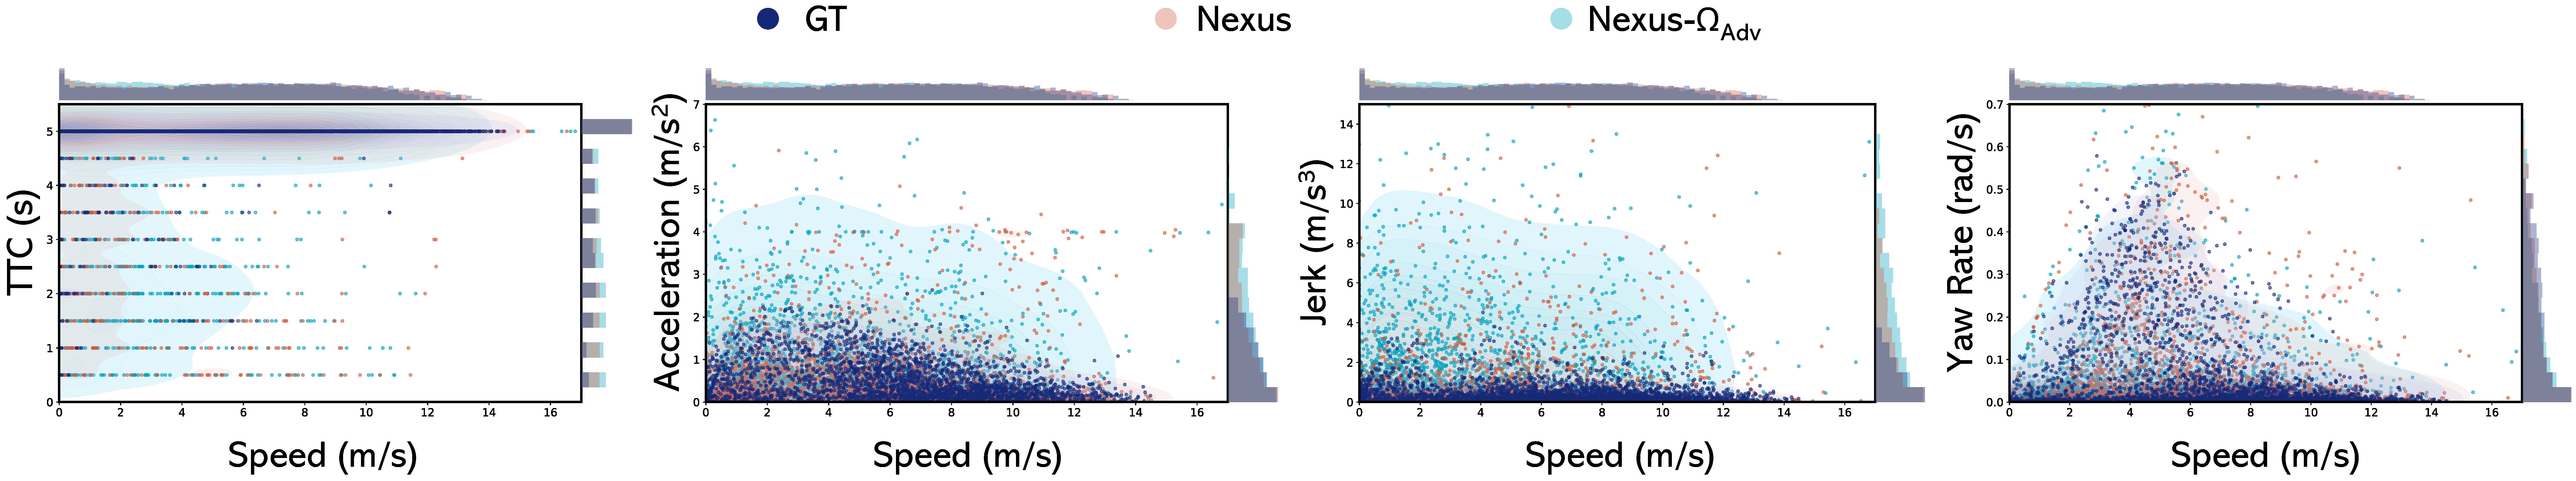
\includegraphics[width=\linewidth]{sec/figs/Distribution.png}
    \vspace{-6pt}
    \caption{
        \textbf{Ego-kinematic distributions in adversarial scenarios.}
        Joint distributions of ego speed with TTC, acceleration, jerk,
        and yaw rate for ground truth (GT), Nexus, and
        Nexus-$\Omega_{\mathrm{Adv}}$.  
        Marginal histograms use a logarithmic scale to emphasize rare
        events. Nexus-$\Omega_{\mathrm{Adv}}$ produces more short-TTC
        frames, shifts ego speeds toward lower and medium ranges, and
        broadens acceleration and jerk distributions, indicating
        stronger adversarial effects on ego motion.
    }
    \label{fig:adv_dist}
\end{figure*}

\paragraph{Complete numerical results}
Tables~\ref{tab:controllability_full}, \ref{tab:guidance_comparison_full},
and \ref{tab:ablation_full} report the complete quantitative results
for the goal-conditioned controllability experiments, the
comparison with alternative guidance strategies, and the ablation
study performed under the free-exploration setting, including all distributional JSD metrics as well as both per-agent and per-scene validity statistics.  
All metrics follow the definitions in \cref{sec:protocols_metrics}.

The expanded quantitative results confirm the overall trends
reported in the main paper. Across the three evaluation settings,
Nexus-$\Omega$ achieves substantial gains in physical
plausibility, reflected by reduced collisions, fewer off-road
incidents, and higher kinematic feasibility, while preserving strong distributional
alignment with real driving data.  
The full guidance and ablation results further illustrate how the
two-phase schedule and the KL-bounded re-anchoring contribute to
improvements in safety, stability, and cross-agent consistency.

\paragraph{Ego-kinematic statistics in adversarial scenarios}
\cref{fig:adv_dist} visualizes ego-vehicle behavior in the
adversarial generation setting through joint distributions of
speed with TTC, acceleration, jerk, and yaw rate.  
Marginal histograms are plotted on a logarithmic scale in order
to emphasize rare but safety-critical events.

Compared with the pretrained Nexus generator and ground-truth
logs, Nexus-$\Omega_{\mathrm{Adv}}$ produces a markedly higher
density of short-TTC frames, especially within low-to-moderate
speed ranges, indicating that the generated attacker behavior
successfully creates more safety-critical interactions.
The ego speed distribution shifts toward lower and medium
velocities, consistent with defensive slowdowns in response to
adversarial pressure.  
Acceleration and jerk exhibit broader spread across speeds,
reflecting more frequent braking and speed modulation during the
generated interactions.  
The yaw-rate distribution remains comparable to that of Nexus and
ground truth, suggesting that the increased adversarial intensity
primarily manifests through longitudinal rather than lateral
maneuvers.

Overall, these distributions show that OMEGA effectively guides
the generator toward scenarios with higher safety-critical event
density while preserving physically plausible ego responses.


\subsection{Additional Qualitative Results}

\begin{figure*}[!ht]
    \centering
    \includegraphics[width=\linewidth]{sec/figs/Sup_norm_all.pdf}
    \vspace{-10pt}
    \caption{\textbf{Free Exploration on nuPlan.}
\textbf{Top (two rows):} Multiple inference runs on the same initial scene produce diverse scene variations.
\textbf{Bottom (three rows):} Additional examples across varied nuPlan scenarios, illustrating the breadth of freely generated scene variations.}
    \label{fig:Sup_norm}
\end{figure*}

\begin{figure*}[!ht]
    \centering
    \includegraphics[width=\linewidth]{sec/figs/Sup_waymo_full.pdf}
    \vspace{-10pt}
    \caption{\textbf{Zero-Shot Free Exploration on Waymo.}
\textbf{Top (two rows):} Multiple inference runs on the same initial scene produce diverse scene variations.
\textbf{Bottom (three rows):} Additional examples across varied Waymo scenarios, illustrating the broad generalization ability and diversity of freely generated scene variations.}
    \label{fig:Sup_waymo}
\end{figure*}


\begin{figure*}[!ht]
    \centering
    \includegraphics[width=\linewidth]{sec/figs/Sup_goal_full.pdf}
    \vspace{-10pt}
    \caption{\textbf{Goal-Conditioned Scene Generation.}
\textbf{Top (two rows):} Starting from the same initial scene, manually specifying different goal points for selected agents yields diverse yet consistent goal-directed outcomes. The green flags indicate the user-defined goal locations.
\textbf{Bottom (three rows):} Additional examples across varied nuPlan scenarios, showcasing controllable and coherent behavior generation under different goal specifications.}
    \label{fig:gc}
\end{figure*}

\begin{figure*}[!ht]
    \centering
    \includegraphics[width=\linewidth]{sec/figs/Sup_adv_all.pdf}
    \vspace{-10pt}
    \caption{\textbf{Adversarial Scene Generation.}
\textbf{Top (two rows):} Varying attacker identities and multiple inference runs yield distinct adversarial outcomes from the same initial history.
\textbf{Bottom (three rows):} Additional examples across diverse scenarios and attacker types, where Nexus-$\Omega_\mathrm{Adv}$ adapts to each attacker’s relative position and automatically generates contextually plausible attack behaviors}
    \label{fig:Sup_adv}
\end{figure*}

\begin{figure*}[!ht]
    \centering
    \includegraphics[width=\linewidth]{sec/figs/Sup_failure.pdf}
    \caption{\textbf{Failure cases of guided scene generation.}}
    \vspace{-10pt}
    \label{fig:Sup_fail}
\end{figure*}

We provide extended qualitative visualizations to complement the
quantitative results. \cref{fig:Sup_norm}--\ref{fig:Sup_adv}
showcase OMEGA's behavior across diverse road layouts, traffic
densities, and task settings.

\paragraph{Free exploration on nuPlan}
\cref{fig:Sup_norm} shows additional qualitative results for
the free-exploration setting on nuPlan. For several scenes, we display
multiple stochastic samples generated from the same historical
initialization to illustrate the diversity of plausible futures
produced by OMEGA while preserving coherent multi-agent interactions.
We also include examples from a wide range of road geometries such as
straight roads, multi-lane segments, intersections, and merging areas,
each presented with one generated sample to highlight performance
across different map structures.

\paragraph{Free exploration on Waymo}
\cref{fig:Sup_waymo} provides complementary visualizations
for the zero-shot setting on Waymo. As with nuPlan, we show multiple
samples for a fixed scene together with a broader set of scenes that
highlight OMEGA's generalization to an unseen dataset with distinct
map geometries and traffic patterns.

\paragraph{Goal-conditioned generation}
\cref{fig:gc} presents extended results for
goal-conditioned controllability. For a fixed scenario, we display
multiple goal specifications for the ego and selected surrounding
vehicles, illustrating how OMEGA adapts trajectories to reach
distinct target states while maintaining interaction coherence.
Additional scenes across different road structures further show
consistent goal satisfaction and physically plausible multi-agent
coordination.

\paragraph{Adversarial scenario generation}
\cref{fig:Sup_adv} presents qualitative results for adversarial
scenario generation. For the same historical initialization, selecting
different vehicles as the designated attacker leads to distinct
adversarial outcomes. These variations arise from
OMEGA$_\mathrm{Adv}$ adapting its refinement to the motion context of
the chosen attacker and synthesizing attack behaviors that are
consistent with its relative positioning and traffic
conditions. Additional examples cover a wide range of challenging
patterns such as emergency braking, merge-in maneuvers, cut-in events,
and close-approach interactions, demonstrating that the generated
scenes capture rich safety-critical behaviors while remaining aligned
with realistic multi-agent dynamics.


\subsection{Failure cases.}

\cref{fig:Sup_fail} illustrates several situations in which the guided
generative process produces suboptimal behaviors. In the first example,
although the two-phase schedule improves long-horizon stability, the Rolling-Zero refinement remains
autoregressive over physical time. As a result, small per-step
errors can accumulate, producing minor autoregressive drift in
stationary agents. This issue can be mitigated by freezing
truly static background vehicles during sampling or by lightly
finetuning the backbone model under the Rolling-Zero schedule.

The second case stems from imperfections in the history conditioning of
real-world logs, where two agents may already overlap at the initial
state due to perception noise. Since the generative process inherits
this initialization, such collisions cannot always be avoided. This can
be addressed by filtering out scenarios in which the history contains
overlapping agents before generation.

A third situation arises when map information is incomplete or missing.
In these cases, map-aware components of the guidance become inactive and
the refinement relies solely on motion cues, which may lead to
off-road predictions. Ensuring consistent map availability or
incorporating fallback geometric priors can help alleviate this
behavior.

The fourth example illustrates that guided sampling operates within
the representational capacity of the underlying diffusion prior.
When the model proposes highly unrealistic trajectories during
denoising, the guidance step may not fully restore physical
consistency. Improving the backbone model therefore remains an
effective direction for future enhancement.



\end{document}
